\pdfoutput=1
% In particular, the hyperref package requires pdfLaTeX in order to break URLs across lines.

\documentclass[11pt]{article}

% Remove the "review" option to generate the final version.
\usepackage[]{acl}

% Standard package includes
\usepackage{times}
\usepackage{latexsym}


% For proper rendering and hyphenation of words containing Latin characters (including in bib files)
\usepackage[T1]{fontenc}
% For Vietnamese characters
% \usepackage[T5]{fontenc}
% See https://www.latex-project.org/help/documentation/encguide.pdf for other character sets

% This assumes your files are encoded as UTF8
\usepackage[utf8]{inputenc}

\usepackage{booktabs}
% Optional math commands from https://github.com/goodfeli/dlbook_notation.


\usepackage{hyperref}
\usepackage{url}
\usepackage{graphicx}
\usepackage{multicol}
\usepackage{multirow}
\usepackage{subfig}

% This is not strictly necessary, and may be commented out,
% but it will improve the layout of the manuscript,
% and will typically save some space.
\usepackage{microtype}

\input{math_commands.tex}

%%%
\newcommand{\xiang}[1]{\textcolor{red}{[Xiang: #1]}}
%\newcommand{\xiang}{}


\title{
\textit{Lifelong Pretraining}: Continually Adapting Language Models\\ to Emerging Corpora
}


% \title{
% Lifelong Pre-training of Language Models
% }

 

\author{Xisen Jin$^{\dagger1}$ \quad Dejiao Zhang$^2$ \quad Henghui Zhu$^2$ \quad Wei Xiao$^2$ \\
        \textbf{Shang-Wen Li}$^{\ddagger2}$ \quad \textbf{Xiaokai Wei}$^2$ \quad \textbf{Andrew Arnold}$^2$ \quad \textbf{Xiang Ren}$^1$
        \\
        $^{1}$University of Southern California \quad $^{2}$AWS AI Labs\\
\texttt{\{xisenjin,xiangren\}@usc.edu} \quad \\
\texttt{\{dejiaoz, henghui, weixiaow, shangwenl, 
xiaokaiw, anarnld\}} \\
\texttt{@amazon.com}
}



%

% The \author macro works with any number of authors. There are two commands
% used to separate the names and addresses of multiple authors: \And and \AND.
%
% Using \And between authors leaves it to \LaTeX{} to determine where to break
% the lines. Using \AND forces a linebreak at that point. So, if \LaTeX{}
% puts 3 of 4 authors names on the first line, and the last on the second
% line, try using \AND instead of \And before the third author name.

\newcommand{\fix}{\marginpar{FIX}}
\newcommand{\new}{\marginpar{NEW}}
\newcommand{\eg}{\textit{e.g.}}
\newcommand{\setup}{\text{LPT}}

\newcommand\blfootnote[1]{%
  \begingroup
  \renewcommand\thefootnote{}\footnote{#1}%
  \addtocounter{footnote}{-1}%
  \endgroup
}

%\iclrfinalcopy % Uncomment for camera-ready version, but NOT for submission.
\begin{document}


\maketitle
\begin{abstract}
%Pre-trained language models (PTLMs) have achieved state-of-the-art performance over a range of natural language processing tasks. These models are typically trained over a static generic-domain corpus up to a certain date (\eg, a Wikipedia snapshot) and fixed for future applications. However, in practice, data from new domains or later time steps, which both feature an evolving data distribution, may constantly emerge and carry new knowledge. Modeling such emerging knowledge while retaining past knowledge is crucial to downstream task performance over all seen distributions. Towards this goal, we study the problem of lifelong learning an up-to-date language model, where the model visits a sequence of unlabeled corpora from various domains or incremental time steps. We propose two data streams, a domain-incremental \textit{academic papers} data stream and a temporally ordered \textit{social media} data stream for study. Extending from replay memory based lifelong learning approaches, we show that using \textit{dark knowledge} (\eg, attention weights, similarity between examples) of old models for future regularization can be helpful to retaining past performance. We observe positive improvements in some of our experiment setups, while we found the simple experience replay (ER) approach to be very effective as well in general despite its simplicity. We hope our work provides a solid and realistic problem setup and inspires future works to study more powerful approaches. 

Pretrained language models (PTLMs) are typically learned over a large, static corpus and further fine-tuned for various downstream tasks.
% While in an open-ended real-world setup, data from new domains or later time steps constantly emerge and carry new knowledge.
%% by Xiang
However, when deployed in the real world, a PTLM-based model must deal with data distributions that deviate from what the PTLM was initially trained on. %, or newly emerged data that contains out-of-distribution information.
In this paper, we study a \textit{lifelong language model pretraining} challenge where a PTLM is continually updated so as to adapt to emerging data. 
Over a domain-incremental research paper stream and a chronologically-ordered tweet stream, we incrementally pretrain a PTLM with different continual learning algorithms, and keep track of the downstream task performance (after fine-tuning). We evaluate PTLM's ability to adapt to new corpora while retaining learned knowledge in earlier corpora.
% The resulting model is fine-tuned over various downstream tasks to measure retention of past knowledge and acquisition of new knowledge. 
%\xiang{1 sentence to summarize the key findings and takeways.}
Our experiments show distillation-based approaches to be most effective in retaining downstream performance in earlier domains. The algorithms also improve knowledge transfer, allowing models to achieve better downstream performance over the latest data, and improve temporal generalization when distribution gaps exist between training and evaluation because of time.
% We evaluate existing continual learning algorithms, and specifically focus on distillation based approaches, which regularizes the change of ``dark knowledge'' in  models. The approaches not only achieves the best performance, but also dissect dark knowledge that are relevant to forgetting. 
We believe our problem formulation, methods, and analysis will inspire future studies towards continual pretraining of language models.
% We hope our problem formulation, methods, and analysis could inspire future study towards continual learning of language models.

%We propose two data streams, a domain-incremental \textit{academic papers} data stream and a temporally ordered \textit{social media} data stream for study. Extending from replay memory based lifelong learning approaches, we show that using \textit{dark knowledge} (\eg, attention weights, similarity between examples) of old models for future regularization can be helpful to retaining past performance. We observe positive improvements in some of our experiment setups, while we found the simple experience replay (ER) approach to be very effective as well in general despite its simplicity. We hope our work provides a solid and realistic problem setup and inspires future works to study more powerful approaches. 


\end{abstract}
\section{Introduction}
\blfootnote{$\dagger$ Work done during an internship at AWS AI Labs.}
\blfootnote{$\ddagger$ Work done while at Amazon.}
Pretrained language models (PTLMs) have achieved remarkable performance on benchmark datasets for a range of NLP tasks~\cite{Liu2019RoBERTaAR, brown2020language}. 
% However, in an open-ended real-world setup, the distribution of data may constantly shift from that of pretraining corpus, 
However, when deployed in the wild, NLP systems must deal with emerging data that have constantly shifting data distribution, different from the text corpora they were initially pretrained on --- for example, when new data domains are introduced (upper part of Fig.~\ref{fig:datasets})~\cite{Gururangan2020DontSP}, or when the language uses and vocabulary change over time (lower part of Fig.~\ref{fig:datasets})~\cite{Lazaridou2021PitfallsOS}. 
% For example, one may extend LMs pretrained on encyclopedia text~\cite{beltagy2019scibert} to new science domains such as biomedical papers. As another example, one may expect PTLMs over Tweets~\cite{nguyen2020bertweet} to continually improve so that it solves tasks over the latest tweets.
%\xiang{should touch on that fine-tuning supposes to help such adaptation but why it may not be sufficient.}
Fine-tuning from a static and possibly ``outdated" PTLM may limit the model performance on downstream tasks, %especially in the low data settings, 
as the PTLM may no longer provide an effective model initialization~\cite{beltagy2019scibert, Mller2020COVIDTwitterBERTAN}.
% data distribution shift makes the static PTLM a suboptimal weight initialization.
% Therefore, we study approaches to continuously adapt PTLMs whenever new corpus become available, while retaining knowledge from corpora seen earlier.
Here we look to understand whether continuously adapting a PTLM to emerging data can yield gains on various downstream tasks, and how to achieve better downstream performance for such lifelong PTLM adaptation.
% Towards this goal, we propose to study lifelong (continual) pretraining of language models: the language model is sequentially pretrained over several corpora without (or with only a little) re-training over previously seen corpora.
%To simulate these challenging scenarios, 
%Therefore, we study lifelong pretraining of language models over a sequence of text corpora in order to adapt the PTLM to the latest corpus while 


\begin{figure}
    \centering
    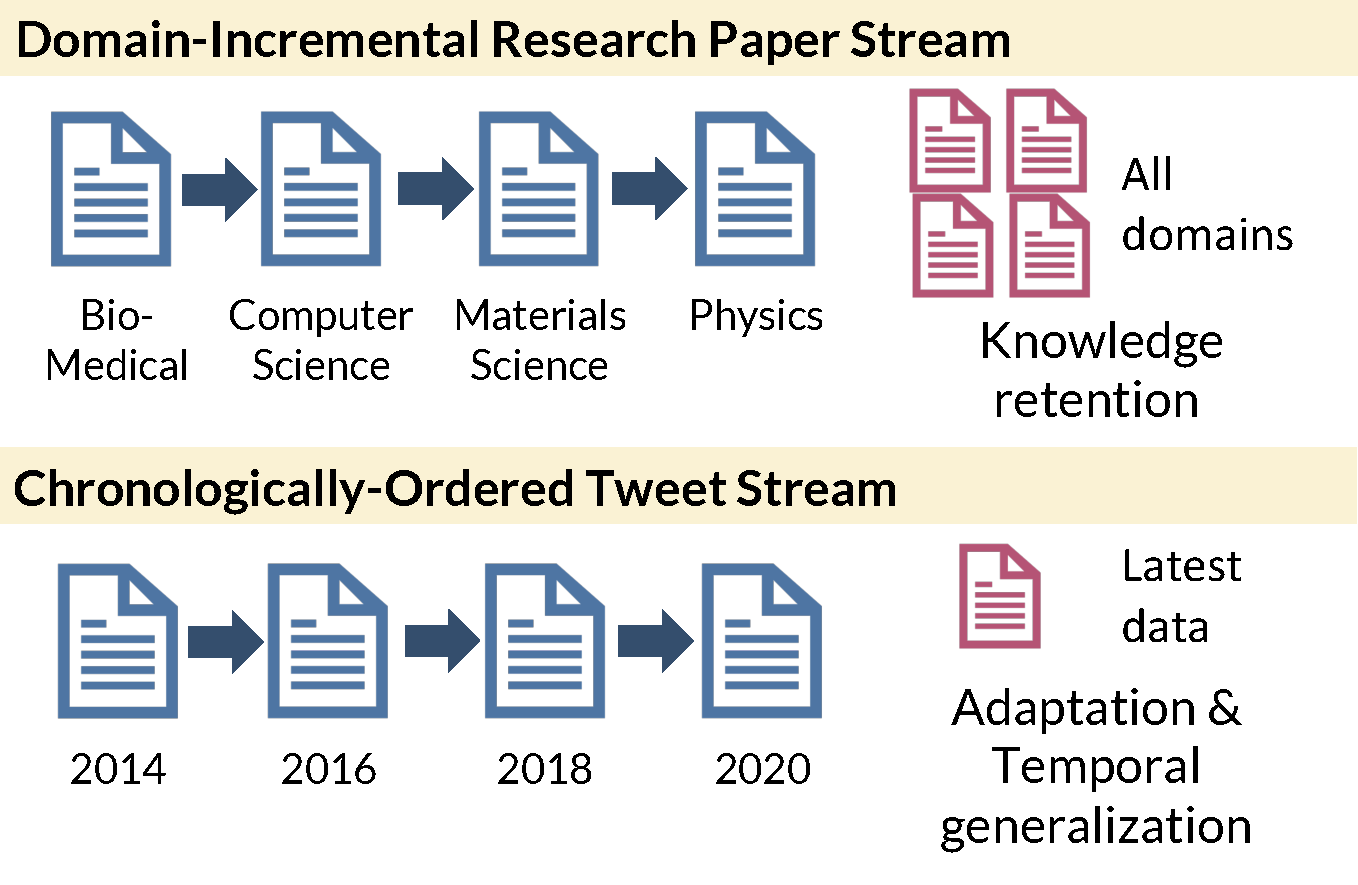
\includegraphics[width=\linewidth]{acl2022/figs/datasets.pdf}
    \caption{Two data streams created for studying lifelong language model pre-training. We focus on evaluating knowledge retention on the domain-incremental research papers stream; we focus on adaptation to the latest data and temporal generalization on the chronologically ordered tweet stream.}
    \label{fig:datasets}
\end{figure}


%\xiang{The current related work paragraph reads a bit vague and weak. I left comments for rewriting.}
A number of recent works make attempts on adapting PTLMs to a new data domain.
\citet{Gururangan2020DontSP, Yao2021AdaptandDistillDS} adapt language models to corpora of different genres and topics
% research papers, news, and product review corpora 
and observe performance improvement in domain-specific downstream tasks.~\citet{Arumae2020AnEI} further show that by regularizing the parameters of PTLMs, the downstream tasks performance on the general domain can be preserved. Another line of works focuses on temporal domain shift~\cite{Hombaiah2021DynamicLM}, which analyzes the effect of pretraining over up-to-date data to the downstream tasks.~\citet{Rttger2021TemporalAO} further study vocabulary composition approaches for improving adaptation to up-to-date corpora.
%In summary, most of existing findings partially address the question on ``\textit{whether adapting PTLMs to a target domain is useful}", through evaluating downstream performance on the target domain. 
However, these work focus their study on adapting PTLM to a single new domain; while in practice, corpora from distinct domains and time stamps may emerge sequentially. 
Whether one can maintain a single, up-to-date PTLM remains an open problem. 
% However, these studies are limited to studying adaptation to only \textit{one} new domain; 
Related to this,~\citet{Lazaridou2021PitfallsOS} study adaptation of PTLMs over temporal data streams, but solely focus on language modeling instead of fine-tuning performance. %investigate the fine-tuning performance on downstream tasks.
% While~\citet{Rttger2021TemporalAO, Hombaiah2021DynamicLM} study the effect of sequential pretraining to downstream tasks, each of them only focuses on a specific metric of success (\textit{e.g.}, downstream performance over latest data). Besides, beyond the analysis, addressing the challenge from a modeling and continual learning perspective has been missing.
It is also important to understand multiple aspects of the utility of lifelong PTLM pretraining, such as knowledge retention over all the seen data, and study what methods can improve the utility of PTLMs in such a continual pretraining process.


%However, continual (sequential) pretraining over multiple distinct corpora is less studied --- it is unclear how the LM can continually acquire and accumulate knowledge from different corpora to benefit downstream tasks in a new domain or on more recent data, and whether the LM can retain the knowledge learned from earlier corpora to preserve decent performance on seen domains. 

% and the forgetting happens to earlier intermediate corpora is less studied.

% While there are abundant prior works on continual learning~\cite{Sun2020LAMOLLM, Kirkpatrick2017OvercomingCF}, 
%\xiang{I think this paragraph needs to be revised and moved after we introduce the analysis workflow and questions (the next paragraph). We can merge this into the method paragraph you currently have, to talk about what are the technical challenges and what methods we examines/compare and how we tweak things to try to resolve the challenges.}
%Furthermore, lifelong LM pretraining poses unique challenges to existing continual learning (CL) methods. 
%For memory-based CL approaches~\cite{Wang2019SentenceEA, chaudhry2019tiny}, a small number of training examples may not be sufficient to represent past knowledge that should be retained, as the size of the pretraining corpus is typically huge. Moreover, there is no guarantee that a CL approach that retains pretraining performance also retains fine-tuning performance well, as the latter solely depends on the learned representations instead of the masked language modeling prediction head. 
% In addition, the focus of evaluation in continual pretraining closely relates to practical use cases: for example, in continual pretraining over multiple text domains, retention of knowledge and less catastrophic forgetting is crucial to the aggregated multi-domain performance; while in continual pretraining over temporal data, it is more crucial how the model performs on the latest data.



In this paper, we formulate a \textit{Lifelong Language Model Pretraining} task to simulate practical scenarios of maintaining and adapting a PTLM over emerging corpora, create a testbed (along with pretraining data streams and downstream tasks) for studying continual pretraining algorithms, and present a systematic evaluation protocol for measuring the progress made on this challenging problem (see Figure~\ref{fig:problem} for an illustration). 
% \xiang{need update.}
We consider two types of text corpus sequences when constructing pretraining data streams, each of which simulates a representative use case and that has slightly different focuses on the evaluation: continuously learning a single model that is applicable to both old and new domains; and improving the model's ability to handle latest data.
%\xiang{needs some rewriting for the below sentence to better clarify the focus and distinctions}
% with major difference in their goals: 
%knowledge retention over all past data, or adaptation to the latest data.
Specifically, we construct
1) a domain-incremental text stream that consists of academic papers published in four research fields, and
2) a temporal tweet stream that consists of tweets collected from four different years.
% Depending on the data stream, 
By conducting systematic experiments on these two data streams,
we look to answer a series of analysis questions: 1) whether continual pretraining retains fine-tuning performance over earlier corpora compared to traditional offline pretraining, 2) whether pretraining improves downstream performance on the latest data, and 3) whether pretraining improves temporal generalization where training and evaluation have distribution gaps because of time.
%\xiang{Expand to include more on the measures of success we're focusing on when answering the above questions -- i.e., what mean good or bad to us?}
%\xiang{Revise to better reflect 1) the ability of PTLMs we look to examine in this task setting; 2) the corresponding analysis questions we asked for the capability above and how we setup the analysis to get answers; and along with 3) the quantitative measurement we focus on for examining the ability.}
%We keep track of the downstream task performance of fine-tuned models and focus on the evaluation of knowledge preservation on the domain-incremental text stream; while for the chronologically ordered stream, we focus on adaptation to latest data and temporal generalization where training and testing distributions are from different time steps in downstream tasks.
%We evaluate fine-tuning performance of downstream tasks selected from earlier works for the research paper stream; while for the tweet stream, we construct downstream datasets using tweets from each year. These downstream datasets allow us to quantify knowledge retention, catastrophic forgetting, and adaption ability of continually pretrained models. 
%\xiang{revise this paragraph a bit to present the analysis questions we look to answer through the experiments.}
%\xiang{say a bit more on the motivation of the following study first.}
%\xiang{Improve this para to 1) smooth out the transition and 2) say more on why this is a non-trivial tech problem and its relation to existing efforts on CL methods (e.g., are existing methods enough? why existing methods may not be effective here;).}
%We further provide extensive analysis on distillation based approaches, integrating various knowledge distillation techniques to continual learning, to dissect the research question - which ``dark knowledge'' should be retained to best improve overall pretraining performance.



%\xiang{Update according based on the analysis questions we asked in earlier paragraph.} % need to be updated based on the latest exp results on twitter
%\xiang{Enrich RE analysis questions above.}
% We try to figure out the best working approach to continually pretrain language models.
To address the research questions above, we conduct a systematic evaluation of existing continual learning (CL) algorithms, spanning over model-expansion based, memory-based, and distillation-based approaches. 
Our results show distillation-based approaches are most effective in knowledge retention in the research paper stream, while simultaneously improve adaptation to latest data and temporal generalization in the tweet stream.
%Our results show that, 1) continual learning algorithms are effective for knowledge retention, where distillation-based approaches perform the best; 2) at the same time, continual pretraining improves adaptation to latest data and temporal generalization.% but does not improve adaptation to latest data on the tweet stream.
We believe our problem formulation, evaluation setup, methods and analysis can inspire more future work on continual pretraining of language models.


\section{Problem Formulation}
\label{sec:setup}Here we present the problem formulation for lifelong pretraining of PTLM, provide details about the data stream construction process and downstream tasks, and introduce the evaluation protocol.

% \xiang{Please work out 2 more illustrative figures:
% 1) One for illustrating the two different data streams + what we want to evaluate/analyze on the stream;
% 2) one for side by side comparing the CL baselines and KD variants}



\subsection{Lifelong Pretraining of PTLMs}
% We consider the scenario where a pretrained language model $f$ visits a sequence of $T$ (unlabeled) text corpora $D_{1..T}=\{D_1, D_2,...D_T\}$, indexed by $t$. 
We consider the scenario where one needs to deploy and/or maintain NLP models over a sequence of $T$ data domains. At each time step $t$ the model visits an unlabeled text corpus $D_t$ from a domain with a data distribution $P(D_t)$. The data distribution $P(D_t)$ evolves as the time step $t$, forming a \textit{data stream} $D_{1..T}=\{D_1, D_2,...D_T\}$. In practice, the data domain shift can refer to the topic change of the text content (from computer science research papers to biomedical papers), or temporal evolution of the text (from past to recent tweets).
The task of \textit{lifelong pretraining of PTLM} looks to continuously adapt a language model $f$ as the model visits (unlabeled) text corpus $D_t$ from the data stream $D_{1..T}$, in order to provide a good model initialization for fine-tuning on downstream tasks from the same domain. With slight abuse in notations, we also use $D_t$ to directly refer to a data domain. 

%Here, we refer to each corpus $D_t$ as a pretraining  for the language model $f$ to learn.
%Here, we also use $D_t$ to refer to the domain of the corpora for the language model $f$ to learn.
Here, we assume a language model $f$ is updated sequentially over each pretraining corpora $D_t$, without accessing the full earlier corpora $\{D_i\}_{i<t}$ in the data stream $D_{1..T}$. This aims to capture practical constraints such as privacy restriction for storing earlier data, or computation budget for training over all the text corpora in $D_{1..T}$. 
% is trained over each task, while it is prohibited to access or retrain over the full corpora from earlier tasks. The constraint is common in practice, \eg, because of privacy issues to store earlier datam and time/computation budget for retraining over all previous corpora. 
We use $f_t$ to denote the language model right \textit{after} updating on the domain $D_t$. 
In our study, $f$ is a RoBERTa-base transformer~\cite{Liu2019RoBERTaAR} and the model ($f_0$) is initialized with pretrained RoBERTa weights.

The utility of the PTLMs $\{f_t\}$ is evaluated based on their fine-tuned model performance on various downstream tasks. 
After updating on a domain $D_{i}$,
the model $f_{i}$ can be fine-tuned over downstream tasks from visited domains $D_t$ where $t \leq i$. We note the set of downstream tasks related to domain $D_t$ as $S_t = \{S_t^j\}_{j=1}^{N_t}$, assuming the number of downstream tasks is $N_t$. %$\{D_{t,j}^{\textrm{FT}}\}$ %\xiang{needs update throughout the paper}, 
% where $t$ denotes that the downstream task is related to $D_t$ and 
%The resulting fine-tuned models are further evaluated on the corresponding held-out test sets of the downstream task to help assess the model performance (more details in Sec.~\ref{ssec:evaluation_protocols}). 
%We note the performance of the fine-tuend models on the downstream task $S_t$ from a pretrained model $f_i$ as $s(f_i, S_t)$.
Note that in the fine-tuning stage, model $f_t$ has no access to any of the pretraining corpus $D_{1..T}$. 


\begin{figure}
    \centering
    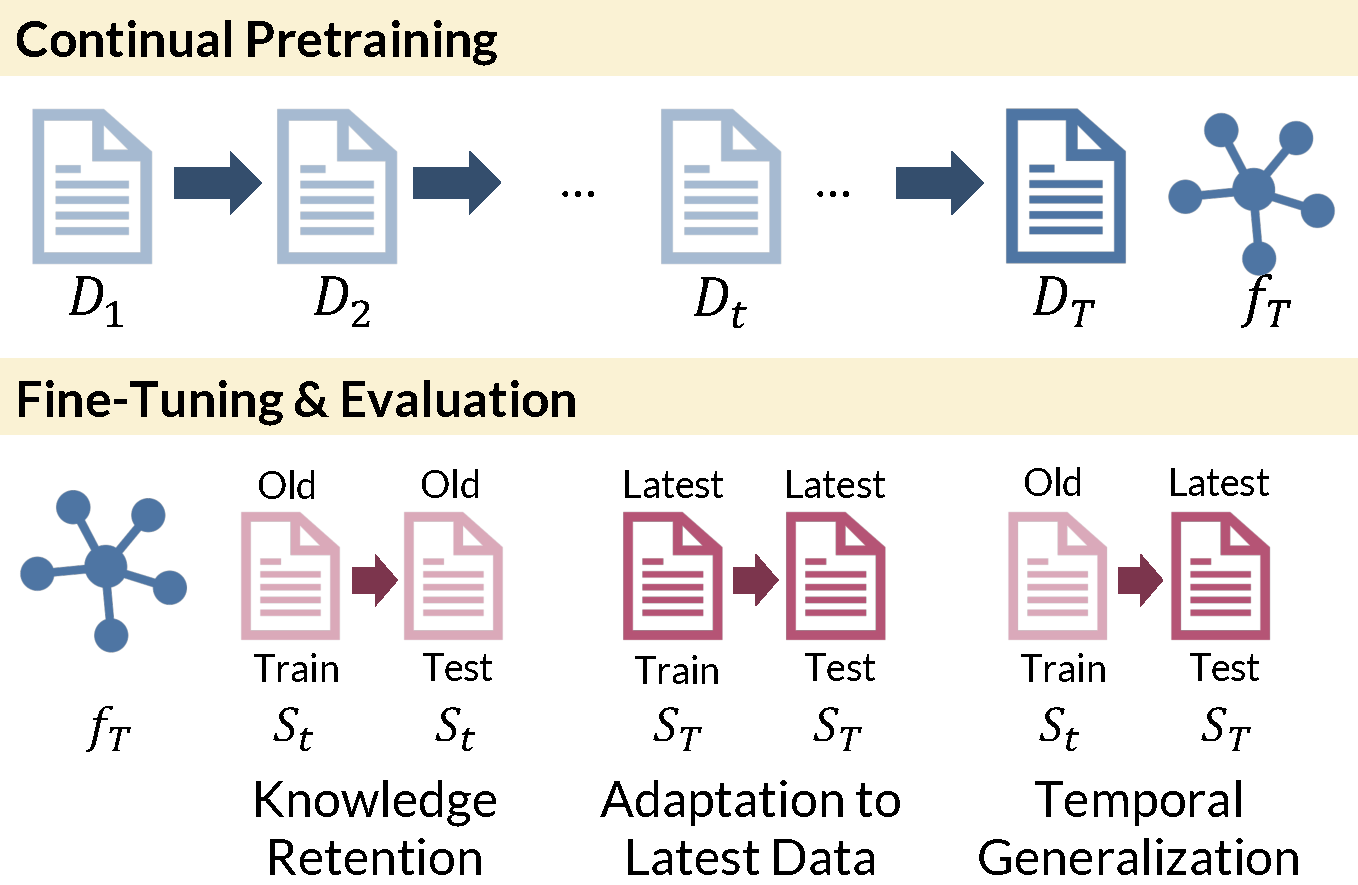
\includegraphics[width=\linewidth]{acl2022/figs/problem.pdf}
    \caption{\small \textbf{Training, evaluation setups, and metrics of lifelong language model pretraining.} The model sequentially visits each corpus, and is fine-tuned on downstream datasets related to the domains of pretraining. We evaluate knowledge retention and adaptation to new data with downstream fine-tuning performance on old and latest domains respectively. Besides, we evaluate temporal generalization where training/test examples are drawn from different time steps.
    %\xiang{need more explanation to make this figure's msgs sefl-contained. For example, I don't quite get the ``knowledge retention" and ``adaptation" part by just looking at the figure.}
   % \xiang{need to update the notations of downstream datasets.}
    }
    \label{fig:problem}
\end{figure}


\vspace{-0.1cm}
\subsection{Data Streams \& Downstream Datasets}
\label{ssec:datasets}
We construct data streams to simulate two representative scenarios of data domain shifts in practice (also see Fig.~\ref{fig:datasets}): one \textit{domain-incremental} stream to simulate the sequential changes of research paper areas; and one \textit{chronologically-ordered} stream to simulate tweets emerging over time.
% namely a domain-incremental research paper stream and a chronologically-ordered tweet stream. 
% Figure~\ref{fig:datasets} illustrates the created data streams and the evaluation focus of two data streams.


\paragraph{Domain-incremental Paper Stream.} This paper stream consists of the full text of research papers published in four research areas: biomedical, computer science, material science, and physics, filtered from the S2ORC dataset\footnote{\scriptsize{We use the 20200705v1 version of the S2ORC dataset at \url{https://github.com/allenai/s2orc}}}, which are presented sequentially to the model. For each domain, we evaluate downstream performance over two datasets. The downstream tasks span over various tasks such as relation extraction and named entity recognition, and are summarized in Table~\ref{tab:academics_downstream}. We detail these datasets in Appendix~\ref{apdx:dataset_details}. %(stat in progress)
%\xiang{any stats about \# papers in each area? Are they randomly sampled or sth else?}



\paragraph{Chronologically-ordered Tweet Stream.} 
This tweet data stream consists of tweets from the year 2014, 2016, 2018 and 2020, collected by the Archive Team\footnote{\scriptsize{\url{https://archive.org/details/twitterstream}}} and preprocessed following~\citet{nguyen2020bertweet}. These four tweet corpora are presented sequentially to the language model following the chronological order of the tweet year.
%We pre-processed the tweets by converting user names and urls to the special USER token and URL token respectively following %\xiang{why so? say a bit more}. 
For downstream tasks, we hold out 1M tweets from each year's corpus to construct multi-label hashtag prediction datasets~\cite{Gong2016HashtagRU} and single-label emoji prediction datasets~\cite{Barbieri2018SemEval2T}. On two datasets, we report label ranking average precision scores (a multi-label version of MRR) of models ~\cite{Azeemi2021COVID19TA} and Macro-F1 respectively. The detailed dataset construction process is included in Appendix~\ref{apdx:dataset_details}. 
%The label space consists of tweets containing 200 most frequent hashtags in each year. 
%We independently sample 500 tweets per label (hashtag) as training, validation and test sets, which results 10$k$ examples in each of the data splits. We also construct a 20-way single-label emoji prediction datasets following~\citet{Barbieri2018SemEval2T} with the 1M held out tweets with 5,000 tweets per emoji in each split.%, resulting in balanced datasets of the same size as the hashtag prediction datasets.
%\xiang{add a line to point to appendix for more details on the dataset construction and the full list of hashtags used in our exps.}



\subsection{Evaluation Protocol}
\label{ssec:evaluation_protocols}

% Our evaluation protocols are designed to benchmark practical usage of approaches in two axes: knowledge preservation of earlier data as well as adaptation and generalization ability to latest data.
We consider three key aspects for evaluating the utility of the language models $\{f_t\}$ that are continuously updated over the data stream $D_{1..T}$, also illustrated in Figure~\ref{fig:problem}: 
1) knowledge retention and transfer over the pretraining corpora seen earlier; 2) adaptation to the latest data domain, and 3) temporal generalization when training and evaluation data are from different time steps.

%\xiang{This subsection needs some careful revision/rewriting to clarify things and align with current analysis.}

\paragraph{Knowledge Retention.} 
%\xiang{better to first provide the high level ideas on what this aspect is about, before diving to the specific stream.}
A key utility of continual language model pretraining is to obtain a single model applicable to all domains. We focus on the evaluation of the ability with the domain-incremental paper stream, because for the tweet stream, the practical need of performance over outdated data is limited. Knowledge retention is measured with the downstream task performance from earlier or the current domains that the pretrained model has visited. More formally, for each pretrained model checkpoint in $\{f_i\}$, we fine-tune $f_i$ over downstream tasks $\{S_t\}$ where $t\leq i$ and evaluate the corresponding test set performance. It is important that the models do not suffer from catastrophic forgetting~\cite{Robins1995CatastrophicFR}, \textit{i.e.,} significantly reduced helpfulness when $f_i$ is fine-tuned for downstream tasks $S_t$ from earlier domains with $t<i$. 
%\xiang{should mention knowledge transfer too, since this is part of our analysis.}
%One major challenge in such use case is the catastrophic forgetting, \textit{i.e.,} significant performance degrade over seen domains To evaluate knowledge retention, we fine-tune a language model $f_{t}$ over downstream tasks $D_{t^\prime,j}^{\textrm{FT}}$, for each domain $t=1, ..., T$.
% from all previously seen domains. 
%We use $s(f_{t}, D_{t^\prime,j}^{\textrm{FT}})$ to denote the performance of the model fine-tuned from $f_{t}$ on $D_{t^\prime,j}^{\textrm{FT}}$. 
%\xiang{below are hard to follow; try rewrite and expand with more clear description, using notations.}
%We track the performance of the fine-tuned model on a dataset %$D_{t^\prime,j}^{\textrm{FT}}$ over the pretraining time steps $t$ ($t^\prime \leq t \leq T$) and inspect the change of the performance. 
%The forgetting is indicated by the performance degrade over the time step $t$.
%\xiang{what about knowledge transfer aspect?}% <--- this is more related to performance on latest data (below)


\begin{table}[]
\centering
\scalebox{0.65}{
\begin{tabular}{@{}llc@{}}
\toprule
Domains           & Downstream Datasets                       & Metrics  \\ \midrule
Bio-Medicine      & Chemprot~\cite{Vindahl2016ChemProt30AG}   & Micro-F1 \\
                  & RCT-Sample~\cite{Dernoncourt2017PubMed2R} & Micro-F1 \\
Comp. Science  & ACL-ARC~\cite{Jurgens2018MeasuringTE}     & Macro-F1 \\
                  & SciERC~\cite{Luan2018MultiTaskIO}         & Macro-F1 \\
Mat. Science & Synthesis~\cite{mysore2019materials}      & Macro-F1 \\
                  & MNER~\cite{olivetti2020data}              & Micro-F1 \\
Physics           & Keyphrase~\cite{augenstein2017semeval}    & Macro-F1 \\
                  & Hyponym~\cite{augenstein2017semeval}      & Macro-F1 \\ \bottomrule
\end{tabular}
}
\caption{Summary of downstream datasets relevant to each domain in the research paper stream.}
\label{tab:academics_downstream}
\vspace{-0.2cm}
\end{table}

\paragraph{Adaption to Latest Data Domain.} 
%\xiang{I think adaption is not only for tweet stream. Currently the writing mislead me about this.}
In certain scenarios, performance of downstream models over the latest data domain should be emphasized. For example, classifiers in the tweet domain are usually trained and evaluated with up-to-date data for practical deployment. Formally, we focus on the downstream task performance of models fine-tuned from the final pretrained model checkpoint $f_T$, where the downstream tasks $S_T$ are also from the latest domain. To succeed in these metrics, it is crucial for the model to transfer knowledge from earlier domains to the latest domain. 

%Over chronologically ordered data streams such as the tweet stream, it is more crucial that the model performs well over the up-to-date data instead of outdated data. 
%For this purpose, we focus on evaluating the performance on the downstream dataset $D^{\text{FT}}_{T,j}$ with the latest time step. \xiang{unclear to me.}

\paragraph{Temporal Generalization Ability.}
We consider another practical fine-tuning scenario in the tweet stream where the model is trained on outdated data and evaluated on the latest data~\cite{Rijhwani2020TemporallyInformedAO, Huang2018ExaminingTI}, referred to as the \textit{temporal generalization} ability. %The setup is prevalent to systems deployed online where collecting annotations for always up-to-date data is costly. 
Formally, we fine-tune the final pretrained model checkpoint $f_T$ over the training set of downstream tasks $S_t$ from an earlier time step ($t < T$), and evaluate on the test set of the downstream tasks $S_T$ from the latest time step $T$.
%the model is fine-tuned on outdated training examples, but evaluated on the latest test examples. 



%However, we still report performance of $f_T$ on earlier data for reference. We also evaluate whether $f_T$ improves temporal generalization ability of the model


% \textbf{Challenges}. We summarize several challenges in continual language model pretraining compared to regular continual learning. (1) first, the amount of training data is huge, which may reduce the performance of memory-replay based continual learning algorithms (2) the forgetting that happens in intermediate representations may be more crucial to the fine-tuning performance, so that continual learning algorithms that operates over model outputs may be less effective. In addition, the large output space makes it prohibitive to apply certain knowledge distillation based approaches.



\section{Methods}
\label{sec:methods}

Lifelong language model pretraining introduces novel challenges because of the large training sets and more comprehensive evaluation protocols compared to classification tasks. 
%\xiang{Here is a good place to expand the discussion on technically why this creates unique challenges as compared to CL methods applied to supervised learning.}
We establish several strong baselines, and evaluate the performance of continual learning algorithms from different categories spanning over model-expansion, memory-based, and distillation-based approaches, We illustrate the approaches in Figure~\ref{fig:method}. 

\vspace{-0.1cm}
\subsection{Simple Baselines}
\vspace{-0.1cm}
%\xiang{1) use notations to help clarify; 2) explain and motivate the purpose of including these baselines --- what insights can be brought out when comparing between them.}
We consider several simple baselines which continual learning algorithms will be compared against. \texttt{RoBERTa-base} ($f_0$) corresponds to not pretraining on any of the domain-specific corpora. By separately pretraining $f_0$ on each corpus $D_1,D_2,...D_T$, we obtain $T$ \texttt{Task-Specific} pretrained models. 
%While domain-specific models do not suffer from forgetting, they prohibit knowledge transfer between domains. 
We also pretrain $f_0$ sequentially over $D_{1..T}$, which we refer to as \texttt{sequential pretraining}. While it allows knowledge transfer between domains compared to domain-specific models, without any continual learning algorithms, sequential pretraining is prone to catastrophic forgetting~\cite{Robins1995CatastrophicFR}. Finally, we randomly shuffle corpora from all domains $D_{1..T}$ before pretraining, noted as \texttt{Multi-Task Learning (MTL)}. MTL corresponds to an offline training paradigm that models new corpora by re-training over all corpora seen before. The drawback is that it requires storing full data from earlier domains, and that it can be extremely costly to repetitively retrain over earlier data if new data keeps emerging.
%\xiang{Vanilla method is totally skipped for explanation? Which seems important because all the CL methods add on to it?}
%We also train one task specific model for each domain, noted as \texttt{Task-Specific Models}. As there can be either positive or negative knowledge transfer from other tasks, there is chance that task specific models outperform continually pretrained models.

%\xiang{multi-task learning as the reference baseline.}
%\xiang{introduce the other simple baselines we consider in the study, and also mention about the domain-specific model (``single") as a reference number (upper bound?)}

\begin{figure}
    \centering
    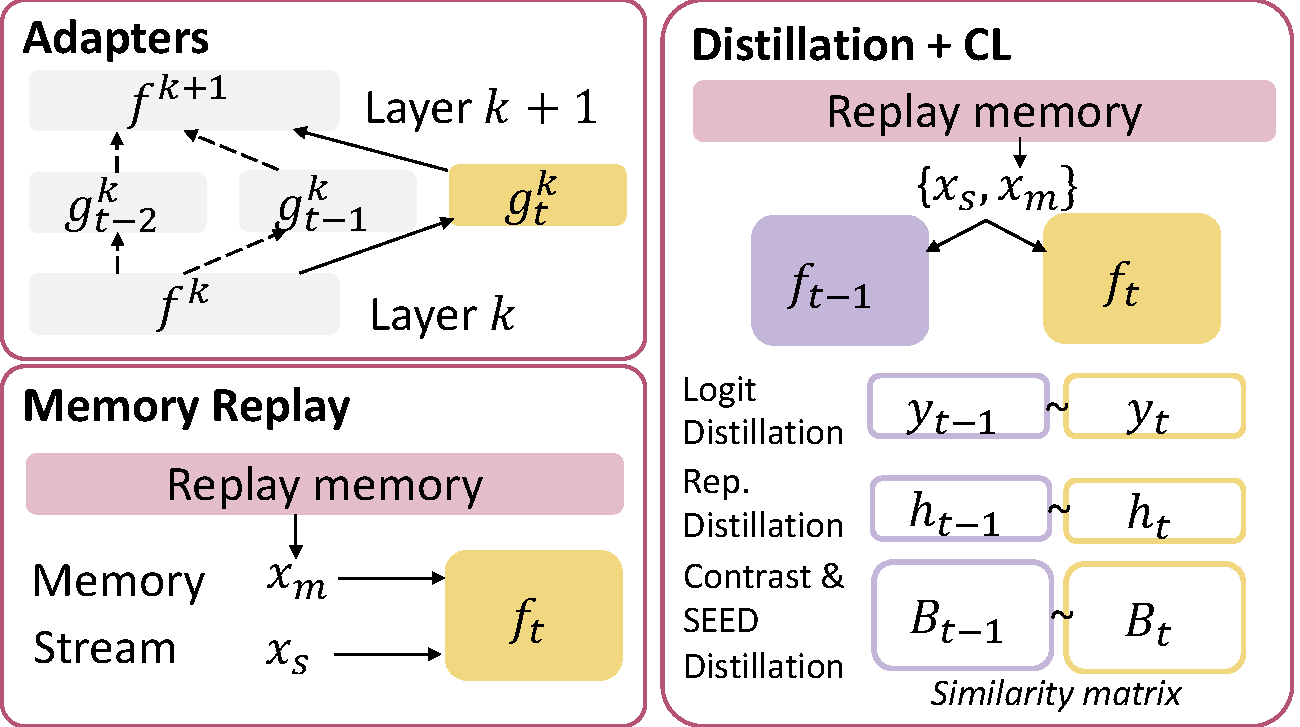
\includegraphics[width=\linewidth]{acl2022/figs/method.pdf}
    \caption{\textbf{Comparison of adapter, memory replay, and distillation-based continual learning algorithms.} 
    Details of the methods are introduced in Sec.~\ref{sec:methods}.
    %We use $g_{t}^k$ to represent adapters created for the task $t$. $\bm{x}_m$ and $\bm{x}_s$ note for the mini-batch of examples drawn from the memory and the data stream respectively.
   % \xiang{Good to include illustration on the three simple baselines.}
    }
    \label{fig:method}
\end{figure}

\vspace{-0.1cm}
\subsection{Model-expansion and Regularization-based Methods}
\vspace{-0.1cm}
%Model expansion based continual learning algorithms create new modules to model new tasks, while freezing (or discouraging change in) shared modules between tasks to prevent interference. It is non-trivial to adapt the approach to large transformer models as most of the algorithms causes significant growth of the model size. 

%\xiang{Good to have 2-3 sentences first give high level overview for this category of methods (model expansion); also can update to include the layer-specific model expansion method.}
We first introduce model-expansion based approaches, which add small trainable modules (\textit{e.g.,} multi-layer perceptron) to the model per new domain while keeping other parts of the model frozen.
The \texttt{Adapter} approach is a representative approach that learns a set of ``adapter'' layers $g_t = \{g_t^k\}_{k=1}^K$ for each domain $D_t$ and each of the $K$ transformer layers~\cite{houlsby2019parameter}. %The adapter layer is inserted between the transformer layers to modify the outputs of transformer layers $h^\prime_{k}$ as $h_{k} =  g_t^k(h^\prime_{k})$. % We implement the adapters as multi-layer perceptrons while keeping the base transformer model frozen during pretraining. 
%During fine-tuning of the language model, we apply Adapter Fusion~\cite{Pfeiffer2021AdapterFusionNT} to aggregate outputs from adapters learned for all domains $g_{1..T}$.
% allowing knowledge transfer from between domains. 
We also experiment with a simple \texttt{Layer Expansion} approach, which learns separate top two layers of the transformer and the prediction head for each domain. %During fine-tuning, we always unfreeze and fine-tune the entire weights of the model.
We also involve a regularization-based continual learning baseline, online EWC~\cite{Schwarz2018ProgressC}, which directly penalize change of model parameters. 

%. Suppose that the related downstream task is known to the model, the model may discard other adapters and only fine-tune the transformer and the corresponding adapter; while the model may also dynamically weight the output of different adapters in each layer, known as AdapterFusion.

\vspace{-0.1cm}
\subsection{Memory Replay Methods}
\label{ssec:mem_replay_methods}
\vspace{-0.1cm}
%\xiang{2-3 sentences to introduce general ideas of the memory-based approach, before diving to ER method.}
We also experiment with Experience Replay (ER)~\cite{chaudhry2019tiny}, which alleviates forgetting by storing a subset of earlier examples and periodically re-training (replaying) over them. We maintain a fixed-size memory $M$ ($100k$ examples by default) and populate the memory $M$ each time pretraining on a domain $D_t$ finishes with examples in the current domain. We ensure $M$ always contains a balanced sample of examples from all seen domains $D_{1..{t}}$. We replay a mini-batch of examples from the memory every 10 training steps.
%We apply experience replay (ER)~\cite{chaudhry2019tiny}, which alleviates forgetting by maintaining a fixed-size replay memory and regularly draw examples from the memory to replay.\xiang{tech details sound vague to me in the current writing. Need revision.}
%We maintain a memory of 100,000 examples, which are approximately 0.30\% and 0.15\% of training examples in the research paper stream and the tweet stream respectively. We populate the memory when the pretraining over the current task finishes, and randomly select examples from the current task to store in the memory. We ensure the memory always contains a balanced number of examples from all previously seen tasks. We sample a mini-batch from the memory to perform replay every 10 training steps.


\subsection{Distillation-based CL Methods}
While knowledge distillation (KD)~\cite{Hinton2015DistillingTK} techniques have been studied intensively for pretrained language models~\cite{Sun2019PatientKD}, applying them to continual learning has been under-explored outside image classification tasks~\cite{Li2018LearningWF, Rebuffi2017iCaRLIC, Hou2018LifelongLV}. Distillation based CL approaches store one previous model checkpoint of the model (noted as $f_{t-1}$) and regularize the differences between $f_{t-1}$ and the current model $f_t$.
We adapt several existing knowledge distillation techniques to PTLMs and utilize them for continual learning. We note, while individual distillation techniques are not original, their adaptation to CL algorithms can be novel.
%\xiang{below part needs adjustment as it sounds too strong and also not quite supported by exp results.}
%Not only do we expect to improve performance with these algorithms, we also hope to analyze which part of the ``dark knowledge'' in pretrained models are most important for knowledge preservation and adaptation.  %The distillation can be performed over the output logits, intermediate model representations, or leverage other information such as representational similarity between training examples. However, the issues of data-mismatch may arise as the knowledge of previous models are extracted with new data, given that examples from previous tasks are no longer available. However, algorithms show improved performance despite the mismatch issue. Other approaches may further store a small porition of previous examples to address the mismatch issue.
% \paragraph{Overall Workflow.} 

%We build distillation approaches on top of memory replay approaches. 
%Usually, knowledge distillation from a model $f_{t-1}$ requires the full training corpora where $f_{t-1}$ is pretrained on (\textit{i.e,} $D_{t-1}$). However, as CL assumes no access to the full corpora $D_{t-1}$ from earlier time steps, we maintain a memory $M$ (similar to ER) to store a subset of past examples for distillation. 
We perform distillation with examples from the current domain $D_{t}$ and a replay memory $M$ (similar to ER). 
Despite the potential gap between $D_{t}$ and the training data of $f_{t-1}$, the approach allows utilizing more data for distillation. Formally,  
each time the model receives a mini-batch of stream examples $\bm{x}_s$ or a draws mini-batch of memory examples $\bm{x}_m$ from $M$ (both noted as $\bm{x}$), we collect certain outputs of the model (\textit{e.g.}, output logits or intermediate representations) with $f_{t-1}$ and $f_t$. 
%\xiang{I got lost on what data we're operating on for doing the KD. Why do we need memory samples?}
We compute a distillation loss $\ell_{\textrm{KD}}(\bm{x}, f_{t-1}, f_t)$ that penalizes the differences between the model outputs, and jointly optimize it with the masked language modeling loss $\ell_{\textrm{MLM}}$. The final objective is written as $\ell = \ell_{\textrm{MLM}} + \alpha\ell_{\textrm{KD}}$, where $\alpha$ is a hyperparameter to weight the distillation loss. %We introduce several distillation approaches applied below.

%\xiang{can we formalize the general method a bit more with notations here? And the late part will provide more concrete tech details by referencing the notations here.}

\paragraph{Logit Distillation.} In logit distillation~\cite{Hinton2015DistillingTK}, we collect the output logits of $f_t$ and $f_{t-1}$, noted as $\bm{y}_t$ and $\bm{y}_{t-1}$ respectively. The distillation loss is computed as 
$D_{\textrm{KL}}(\bm{y}_t, \bm{y}_{t-1})$, where $D_{\textrm{KL}}$ is the Kullback–Leibler divergence function.
%the KL divergence between $\bm{y}_t$ and $\bm{y}_{t-1}$.

\paragraph{Representation Distillation.} 
We also consider minimizing the representational deviation of sentences between previous and current models~\cite{Sun2019PatientKD, Jiao2020TinyBERTDB}. We extract the representation of each word of two models, noted as $\bm{h}_{t-1}^{1:N}$ and $\bm{h}_{t}^{1:N}$, before the masked language modeling prediction head, where $N$ is the length of the sentence. Then, we compute MSE loss $\vert\vert \bm{h}_{t-1}^{1:N} -  \bm{h}_{t}^{1:N} \vert\vert_2^2$ as the distillation loss.


\begin{table*}[]
\centering
\scalebox{0.60}{
\begin{tabular}{@{}lcccccccccccc@{}}
\toprule
Task          & \multicolumn{3}{c}{$D_1$ - Biomedical} & \multicolumn{3}{c}{$D_2$ - Computer Science} & \multicolumn{3}{c}{$D_3$ - Materials Science} & \multicolumn{3}{c}{$D_4$ - Physics} \\
\cmidrule(r){1-1} \cmidrule(lr){2-4} \cmidrule(lr){5-7} \cmidrule(lr){8-10} \cmidrule(l){11-13} 
Dataset       & Chemprot           & RCT-Sample    &  MLM      & ACL-ARC               & SciERC        & MLM        & MNER                   & Synthesis    & MLM         & Keyphrase         & Hyponym     & MLM     \\ \midrule
Roberta-base  & 82.03$_{\pm 0.7}$          & 78.07$_{\pm 0.7}$    & 1.993      & 64.32$_{\pm 2.8}$             & 79.07$_{\pm 1.6}$     & 2.153        & 83.15$_{\pm 0.3}$              & 91.25$_{\pm 0.6}$        & 2.117     & 66.21$_{\pm 1.0}$         & 67.59$_{\pm 4.5}$    &   2.278  \\
Sequential Pretraining         & 82.09$_{\pm 0.5}$          & 79.60$_{\pm 0.5}$      & 1.654    & 72.73$_{\pm 2.9}$             & 81.43$_{\pm 0.8}$    & 1.807         & \textbf{83.99$_{\pm 0.3}$}              & 92.10$_{\pm 1.0}$    & 1.590          & \textbf{67.57$_{\pm 1.0}$}         & \textbf{74.68$_{\pm 4.4}$}    & \textbf{1.381}    \\
\midrule
ER            & 82.73$_{\pm 0.3}$          & 79.98$_{\pm 0.3}$  & 1.737        & 72.50$_{\pm 1.0}$             & 81.64$_{\pm 1.1}$   & 1.857           &  \textbf{83.99$_{\pm 0.4}$}              & 92.65$_{\pm 0.4}$     & 1.621        & 66.11$_{\pm 1.1}$         & 72.82$_{\pm 4.3}$   & 1.391      \\
Online EWC          & 81.83$_{\pm 0.2}$          & 78.84$_{\pm 0.5}$  & 1.655        & 71.81$_{\pm 2.6}$             & 80.79$_{\pm 0.5}$   & 1.803           &  83.43$_{\pm 0.4}$              & 91.89$_{\pm 0.5}$     & 1.571        & 66.70$_{\pm 0.6}$         & 72.98$_{\pm 6.0}$   & 1.388      \\
Adapter       & 83.30$_{\pm 0.4}$          & 80.41$_{\pm 0.4}$  & 1.417        & 69.32$_{\pm 3.5}$             & 80.22$_{\pm 1.5}$      & \textbf{1.633}       &          83.91$_{\pm 0.3}$         &    91.69$_{\pm 0.6}$    & 1.522           & 66.23$_{\pm 1.4}$         & 69.65$_{\pm 4.5}$   & 1.554     \\
Layer Expansion & 83.74$_{\pm 0.3}$ & 81.10$_{\pm 0.5}$ & \textbf{1.210} & 65.17$_{\pm 2.9}$ & 79.35$_{\pm 0.8}$  &  1.756 & 82.48$_{\pm 0.4}$ & 92.33$_{\pm 1.0}$ & 1.389 &  65.70$_{\pm 1.1}$ &  73.34$_{\pm 3.7}$ & 1.534 \\
Logit-KD      & 83.39$_{\pm 0.4}$          & \textbf{81.21$_{\pm 0.1}$}  & 1.392       & \textbf{73.70$_{\pm 3.4}$}             & 81.92$_{\pm 0.8}$      & 1.699       & 83.96$_{\pm 0.3}$              & 92.20$_{\pm 1.0}$      & \textbf{1.425}       & 64.75$_{\pm 1.1}$         & 71.29$_{\pm 3.6}$   & 1.460      \\
Rep-KD        & 82.34$_{\pm 0.3}$          & 79.59$_{\pm 0.5}$ & 1.684        & 71.17$_{\pm 2.5}$             & 78.78$_{\pm 1.1}$      & 1.810       & 84.13$_{\pm 0.3}$              & 92.02$_{\pm 0.8}$   & 1.585           &      65.96$_{\pm 1.6}$      & 73.93$_{\pm 5.5}$       &      1.389     \\
Contrast-KD   & 82.29$_{\pm 0.5}$          & 79.92$_{\pm 0.4}$  & 1.722        & 71.15$_{\pm 1.1}$             & 80.49$_{\pm 1.6}$    & 1.856         & 83.26$_{\pm 0.4}$              & 92.62$_{\pm 0.7}$   & 1.612          & 65.95$_{\pm 1.7}$         & 72.26$_{\pm 3.1}$   & 1.428     \\
SEED-KD & 82.78$_{\pm 0.3}$ & 80.38$_{\pm 0.4}$ & 1.720 & 69.98$_{\pm 2.4}$  & 81.61$_{\pm 0.7}$ & 1.829 & 82.99$_{\pm 0.4}$ & 92.35$_{\pm 0.7}$ & 1.609 & 65.35$_{\pm 1.0}$ & 74.79$_{\pm 4.1}$ & 1.401 \\ 
SEED-Logit-KD &  \textbf{83.72$_{\pm 0.4}$} & 81.05$_{\pm 0.2}$  & 1.391        & 69.90$_{\pm 4.5}$             & \textbf{83.03$_{\pm 0.6}$}   & 1.703           & 83.28$_{\pm 0.5}$              & \textbf{92.87$_{\pm 1.0}$}     & 1.428        & 65.96$_{\pm 1.5}$         & 71.92$_{\pm 5.5}$    & 1.460    \\ \midrule
Task-Specific LM        & 83.74$_{\pm 0.3}$          & 81.10$_{\pm 0.5}$    & 1.210      & 72.20$_{\pm 2.6}$             & 81.24$_{\pm 1.7}$   & 1.629          & 84.02$_{\pm 0.2}$              & 91.56$_{\pm 0.4}$        &  1.418     & 65.95$_{\pm 1.1}$         & 69.43$_{\pm 4.5}$  & 1.426      \\
MTL           & 82.91$_{\pm 1.6}$          & 80.67$_{\pm 0.4}$   & 1.289        & 69.46$_{\pm 1.8}$             & 81.12$_{\pm 0.8}$  & 1.616        & 83.92$_{\pm 0.3}$              & 92.66$_{\pm 0.6}$     &  1.355        & 65.37$_{\pm 1.6}$         & 73.31$_{\pm 5.2}$  & 1.418 \\  \bottomrule
\end{tabular}
}
\caption{\small \textbf{Results on the Research Paper stream.} We report log perplexity of MLM and the performance of downstream models fine-tuned from the final checkpoint of the pretrained model ($t=4$). Performance of the best performing CL algorithm is marked bold.
%\xiang{1) bold the 2nd best too if there's no stat signifcant difference; 2) mention p-value btw top-1 and top-2 method; 3) use up/down arrows to indicate which way the metrics are better.}
}
\label{tab:academics}
\vspace{-0.2cm}
\end{table*}
% \begin{table*}[]
% \centering
% \scalebox{0.60}{
% \begin{tabular}{@{}lcccccccccccc@{}}
% \toprule
% Task            & \multicolumn{6}{c}{Task 1 - Biomedical}                               & \multicolumn{4}{c}{Task 2 - Computer Science}                 & \multicolumn{2}{c}{Task 3 - Materials Science} \\
% \cmidrule(r){1-1} \cmidrule(lr){2-7} \cmidrule(lr){8-11} \cmidrule(l){12-13} Dataset         & \multicolumn{3}{c}{Chemprot}      & \multicolumn{3}{c}{RCT-Sample}    & \multicolumn{2}{c}{ACL-ARC}   & \multicolumn{2}{c}{SciERC}    & MNER                   & Synthesis             \\ \cmidrule(r){1-1} \cmidrule(lr){2-4} \cmidrule(lr){5-7} \cmidrule(lr){8-9} \cmidrule(lr){10-11} \cmidrule(lr){12-12} \cmidrule(l){13-13}
%  Evaluated After & Task 1    & Task 2    & Task 3    & Task 1    & Task 2    & Task 3    & Task 2        & Task 3        & Task 2         & Task 3       & Task 3                 & Task 3                \\ \midrule
% Roberta-base    & {82.03$_{\pm0.7}$}    & {82.03$_{\pm0.7}$} & {82.03$_{\pm0.7}$} & {78.07$_{\pm0.7}$}  & {78.07$_{\pm0.7}$}  & {78.07$_{\pm0.7}$}     & {64.32$_{\pm2.8}$} & {64.32$_{\pm2.8}$} & {79.07$_{\pm1.6}$} & {79.07$_{\pm1.6}$} & 83.15$_{\pm0.3}$              & 91.25$_{\pm0.6}$             \\
% Naive           & \textbf{83.74}$_{\pm0.3}$ & 82.60$_{\pm0.3}$ & 83.37$_{\pm0.5}$ & \textbf{81.10}$_{\pm0.5}$ & 80.49$_{\pm0.3}$ & 80.63$_{\pm0.3}$ & \textbf{73.71}$_{\pm2.8}$     & 69.93$_{\pm2.2}$     & 82.14$_{\pm1.1}$      & 80.70$_{\pm0.8}$    & 83.34$_{\pm0.3}$              & 92.72$_{\pm1.0}$             \\
% ER              & \textbf{83.74}$_{\pm0.3}$ & 82.96$_{\pm0.3}$ & 83.50$_{\pm0.6}$ & \textbf{81.10}$_{\pm0.5}$ & 80.79$_{\pm0.4}$ & 81.04$_{\pm0.1}$ & 69.92$_{\pm1.6}$     & 69.09$_{\pm2.1}$     & 82.01$_{\pm0.9}$      & 80.59$_{\pm0.2}$    & 83.79$_{\pm0.4}$              & \textbf{93.20}$_{\pm0.2}$             \\
% %Adapter-Single  & {83.68$_{\pm0.3}$} &  {83.68$_{\pm0.3}$} &  {83.68$_{\pm0.3}$} & {80.72$_{\pm0.7}$} & {80.72$_{\pm0.7}$} & {80.72$_{\pm0.7}$}    & {68.02$_{\pm2.6}$} & {68.02$_{\pm2.6}$} & {81.60$_{\pm0.8}$} & {81.60$_{\pm0.8}$} &    {84.15$_{\pm0.3}$}                  &      {91.11$_{\pm0.2}$}                 \\ 
% Adapter  & 83.68$_{\pm0.3}$ & 83.03$_{\pm0.4}$ &  83.19$_{\pm0.6}$      & 80.72$_{\pm0.7}$ & 80.63$_{\pm0.7}$ &     80.64$_{\pm0.5}$      & 73.28$_{\pm3.9}$     &         67.60$_{\pm 5.7}$      & 79.79$_{\pm1.5}$      &    80.10$_{\pm 1.0}$          &    \textbf{83.94}$_{\pm 0.4}$                    &          90.82$_{\pm 3.3}$         \\
% Rep-KD          & \textbf{83.74}$_{\pm0.3}$ &        82.24$_{\pm 1.0}$        &    82.90$_{\pm 0.3}$      & \textbf{81.10}$_{\pm0.5}$ &   80.60$_{\pm 0.2}$   &     80.51$_{\pm0.3}$      &       70.68$_{\pm 2.1}$        &     69.93$_{\pm 2.6}$      &      80.45$_{\pm 1.4}$       &       79.58$_{\pm 0.7}$       &     83.89$_{\pm 0.4}$                   &      92.16$_{\pm 0.6}$          \\
% Contrast-KD     & 83.38$_{\pm0.3}$ &    82.39$_{\pm 0.4}$       &    83.06$_{\pm 0.2}$     & 81.00$_{\pm0.3}$ &      80.39$_{\pm0.4}$      &   80.53$_{\pm 0.4}$     &       75.34$_{\pm 2.1}$       &    69.94$_{\pm 1.9}$       &         80.85$_{\pm 1.1}$       &      \textbf{82.45}$_{\pm 0.9}$        &          83.21$_{\pm 0.3}$          &            92.05$_{\pm 0.4}$           \\ 
% Logit-KD        & \textbf{83.74}$_{\pm0.3}$ & \textbf{83.04}$_{\pm0.2}$ & \textbf{84.12}$_{\pm0.4}$ & \textbf{81.10}$_{\pm0.5}$ & \textbf{81.26}$_{\pm0.4}$ & \textbf{81.19}$_{\pm0.2}$ & 70.72$_{\pm2.7}$     & \textbf{71.38}$_{\pm1.8}$     & \textbf{82.74}$_{\pm0.5}$      & 80.93$_{\pm0.8}$    & 83.54$_{\pm0.2}$              & 92.73$_{\pm1.0}$             \\
% \cmidrule(r){1-1} \cmidrule(lr){2-4} \cmidrule(lr){5-7} \cmidrule(lr){8-9} \cmidrule(lr){10-11} \cmidrule(lr){12-12} \cmidrule(l){13-13}

% Task-Specific LM          & \multicolumn{3}{c}{83.74$_{\pm0.3}$}     & \multicolumn{3}{c}{81.10$_{\pm0.5}$}     & \multicolumn{2}{c}{72.20$_{\pm2.6}$} & \multicolumn{2}{c}{81.24$_{\pm1.7}$} &        84.02$_{\pm 0.2}$                &         91.56$_{\pm 0.4}$              \\
% \bottomrule
% \end{tabular}
% }
% \caption{Performance of downstream models fine-tuned from continually pre-trained language models on the multi-domain research paper stream. Performance of the best performing CL algorithm is marked bold.}
% \label{tab:academics}
% \end{table*}



\paragraph{Contrastive Distillation.}
% \xiang{1) can try to compress down this part by 30\% if possible. Seems a bit too heavy on space; 2) It's important to speak out up front what differences in terms of intuitions this method bring as compared to the other KD methods.}
In addition to output logits and hidden representations, we further look into \textit{representational similarity within a batch of examples} as additional knowledge to distill. The approach is adapted from~\cite{Cha2021Co2LCC}, which is originally studied for supervised image classification tasks. %The approach consists of two components: learning a representation space with unsupervised contrastive learning, and regularize the change of representation similarity between examples.
We briefly introduce the adapted algorithm and leave the details in Appendix~\ref{apdx:cl}.
During continual pretraining, in addition to the language model pretraining objective, we add an unsupervised contrastive learning objective, namely the SimCSE~\cite{Gao2021SimCSESC} objective
%, so that the similarity in the sentence representation better 
to encourage sentence representations to reflect semantic similarities between sentences. Then, we compute the intra-batch representational similarity matrices of sentence representations (\textit{i.e.} between each pair of examples in the mini-batch) with $f_{t-1}$ and $f_t$, noted as $\mathbf{B}^{t-1}$ and $\mathbf{B}^{t}$, and minimize the cross entropy loss $\ell_{\text{distill}} = - \frac{1}{N} \sum_{i=1}^{N} \sum_{j=1}^{N} \mathbf{B}_{ij}^{t-1}\log \mathbf{B}_{ij}^{t}$
%\begin{equation}
%    \label{eq:contrastive_distill}

%\end{equation}.

% We use the $l^2$-normalized representation of the start-of-sequence token at the final layer as the sentence representation, noted as $\bm{h}$. Then, we distill the intra-batch representational similarity from the previous model $f_{t-1}$ to the current model $f_t$. Given a mini-batch of $N$ examples $\bm{x}$, we compute the representational dot-product similarity matrix between normalized sentence representations $\bm{h}$ between each pair of examples with $f_{t-1}$ and $f_t$, noted as $\mathbf{B}^{t-1}$ and $\mathbf{B}^{t}$, where each element $\mathbf{B}_{ij}$ is, 
% \begin{equation}
%     \label{eq:normalize}
%     \mathbf{B}_{ij} = \frac{\exp(\bm{h}_i \cdot \bm{h}_j / \tau)}{\sum_{k=1..N}\exp(\bm{h}_i \cdot \bm{h}_k / \tau)}
% \end{equation}
% where $\tau$ is a temperature hyperparameter. We specify a temperature $\tau_t$ for the teacher model $f_{t-1}$ and a temperature $\tau_s$ for the student model $f_t$ separately. We compute the cross-entropy between $\mathbf{B}^{t-1}$ and $\mathbf{B}^{t}$ as the distillation loss,
% \begin{equation}
%     \label{eq:contrastive_distill}
%     \ell_{\text{distill}} = - \frac{1}{N} \sum_{i=1}^{N} \sum_{j=1}^{N} \mathbf{B}_{ij}^{t-1}\log \mathbf{B}_{ij}^{t}
% \end{equation}

\paragraph{Self-Supervised Distillation (SEED).} SEED distillation proposed by~\cite{Fang2021SEEDSD} has a similar spirit as the contrastive distillation. The only difference is that it distills representational similarity \textit{between the batch and a large set of other examples}. We leave the details of the algorithm in Appendix~\ref{apdx:cl}. %As the number of target examples $K$ can be much larger than the batch size, it allows distillation of richer information by regularizing similarities. During pretraining, the method maintains a fixed-size queue $Q$ to cache examples from the current domain $D_t$. Given a mini-batch of training examples $\bm{x}$, it computes cosine similarity between each pair of examples within the batch $\bm{x}$ and $Q$ with $f_{t-1}$ and $f_{t}$, resulting in two similarity matrices $\mathbf{P^{t-1}}$, $\mathbf{P^t} \in \mathbb{R}^{|B|\times |Q|}$. Similar to the contrastive distillation, the distillation loss is the cross-entropy between two similarity matrices $\mathbf{P}^{t-1}$ and $\mathbf{P}^{t}$ computed in the same way as Eq.~\ref{eq:contrastive_distill}. 
We further combine SEED Distillation%, which empirically performs best in retaining knowledge on the research paper stream compared to Contrastive Distillation and Representation Distillation
with logit distillation and refer to the approach as SEED-Logit Distillation.

% In SimCSE, the positive pair is defined as the representations of the same sentence using different dropout masks, while the negative pairs in the mini-batch consist of representations of different sentences within the mini-batch. Let $z$, $z^\prime$ be two random dropout masks. The SimCSE loss is written as,
% \begin{equation}
% \label{eq:simcse}
% \ell_{\textrm{con}} = - \alpha \log \frac{e^{\textrm{cos-sim}(\bm{h}_i^{z_i}, \bm{h}_i^{z_j})/\tau}}{\sum_{j=1}^N e^{\textrm{cos-sim}(\bm{h}_i^{z_i}, \bm{h}_j^{z_j^\prime})/\tau}}
% \end{equation}
% where $N$ is the number of examples in the mini-batch, $\bm{h}_i^{z_i}$ is the sentence representation of an instance $i$ after dropout, $\tau$ is a temperature hyperparameter, $\alpha$ is weighting hyperparameter to the masked language modeling loss. Following the original work, we use the representation of the start-of-sequence (\texttt{<s>}) token as the sentence representation. 


% \textbf{Regularizing Similarity between Examples}. We collect the subset of task-$t$ examples selected to be stored in the memory right after learning task $t$. We group these examples with a group size equals to the batch size, noted as $B$, and note each group as $X_j = \{\hat{x}_{ij}\}_{i=1}^B$. We compute a pair-wise similarity matrix $M_j^{|B| \times |B|}$ for each group of examples and store them in the replay. In future training, we randomly select a group of examples to replay, while simutaneuously discourage the change of similarity matrix $M^\prime_j$ computed with the current model. More specifically, when a group $X_j$ is chosen for replay, in addition to the MLM loss, we added a KL divergence loss $\ell_{reg}=KL(M_j, M^\prime_j)$ that measures distance betweene similarity matrices. The KL divergences uses the same temperature hyperparemter $\tau$ and Eq.~\ref{eq:simcse}.


% \section{Datasets}
% \subsection{Pretraining datasets}
% \label{ssec:pt_datasets}
% In the current stage of the project, we included three data streams study, namely the academic papers dataset, mixed-domain dataset, and the twitter data stream.

% \textbf{Research papers dataset} consists of open-access research papers from biomedical, computer science, physics and material science domains. The dataset is a subset of S2ORC dataset\footnote{\url{https://github.com/allenai/s2orc}}~\citep{Lo2020S2ORCTS} released under CC-BY-NC 2.0. In our main experiments, we assume the model sequentially visits biomedical, computer science, physics and material science domains

% \textbf{Mixed-domain dataset} consists of four domains: biomedical research papers, computer science research papers, new articles, and amazon reviews, where has been applied in~\citep{Gururangan2020DontSP}. Here, biomedical and computer science research papers are from the same source as above. Realnews dataset~\citep{Zellers2019DefendingAN} is obtained via a google form at~\url{https://github.com/rowanz/grover/tree/master/realnews} and the license is pasted in Table~\ref{tab:license_realnews}. The amazon reviews dataset is a public dataset accessible at~\url{https://nijianmo.github.io/amazon/index.html}.



% \textbf{Twitter Data Stream}. 
% Following~\cite{Nguyen2020BERTweetAP}, we pretrain the model over the twitter data stream grabbed by the Archive Team\footnote{\url{https://archive.org/details/twitterstream}}, ranging from 01/2012 to 04/2020. 

% \subsection{Downstream Fine-Tuning Datasets}
% We fine-tine the models over a number of downstream fine-tuning tasks after pretraining. We summarize downstream datasets applied in Table~\ref{tab:downstream}. In addition, in the future we may construct our own manually labeled dataset over the pretraining datasets (introduced in Sec.~\ref{ssec:pt_datasets})


\section{Results}
We summarize our findings over the created data streams. We ask whether lifelong pretraining and continual learning algorthms are effective base on our evaluation protocol proposed in Sec.~\ref{ssec:evaluation_protocols}. 
%\xiang{Let's post a few high-level analysis questions here to overview the section.}



% \xiang{Need an experiment setting or setup subsection to give some details: 1) eval metrics for different downstream tasks; 2) additional details about data streams and datasets; 3) implementation details, hps config, etc.}
\subsection{Experiment Settings}
We use the \texttt{RoBERTa-base} model~\cite{Liu2019RoBERTaAR}, initialized with RoBERTa-base weights throughout the experiments. We set the maximal sequence length to 128 and an effective training batch size of 2,048. On the research paper stream, models are trained for 8$k$ steps in the first domain and 4$k$ steps in the subsequent domains. On the Tweet stream, we train the models for 4$k$ steps in each domain. These correspond to less than a single pass of data in each domain. See Appendix~\ref{sec:hyps} for detailed setups. %\xiang{below details can move to appendix and leave a pointer here.}


% \subsection{Results on the Research Paper Stream}
\subsection{Domain Incremental Data Stream}
%\xiang{say a few sentences to re-cap the data stream setup and what aspects of model capability (i.e., measure of success) we're looking at here. Next, you can describe the exp setup/workflow as follows.}
As we introduced in Sec.~\ref{ssec:datasets}, in the domain incremental research paper stream, %the criterion is whether models can transfer knowledge to new domains while retaining knowledge in the domains visited earlier. 
we expect a model $f_t$ to perform well on all downstream tasks $S_{1..t}$ from domains $D_{1..t}$.
%\xiang{Still reads a bit vague to me; above can be further clarified using more notations.}
%\xiang{reference notations in Sec 2.1 to clarify more on the exp settings.}
In Table~\ref{tab:academics}, we report the performance of models on all downstream tasks $S_{1..T}$ fine-tuned from the final pretraining checkpoint, $f_T$. 
%For each downstream task related to a domain $D_t$, we fine-tune the language models at the time step $t$ and afterward, as indicated in the header ``evaluated after'' in Table~\ref{tab:academics}. 
We visualize more complete change of downstream task performance over different time steps of pretraining (\textit{i.e.,}, $f_1, f_2,f_3,f_4$) in Fig.~\ref{fig:academics_curve}. We also report the log perplexity of masked language modeling (MLM) in Table~\ref{tab:academics} as additional information. With these results, we address the research questions below.

%Table~\ref{tab:academics} summarizes the fine-tuning performance over the research paper data stream. 

% \xiang{\paragraph{\textit{Q1: Does sequential pretraining help retain knowledge across different domain corpora?}}
% (1) first talk about task-specific LM vs. roberta to show that domain corpus are useful for the corresponding downstream tasks;
% (2) see if Sequential Pretraining bring gains vs. task-specific LM --> if results are mix that mean that sequential pretraining (Sequential Pretraining) has space to be improved.
% }

%\xiang{Do we have anything special to say about MLM? I think the discrepancy between MLM and downstream performance are interesting to speak out?}

%\xiang{I don't see Fig~\ref{fig:academics_curve} being analyzed in details in any part now? I expect some interesting insights can be derived there.}

\paragraph{\textit{Does lifelong pretraining help retain knowledge across different domain corpora?}}
We first examine whether task-specific or lifelong pretraining improves performance over domain-specific downstream tasks. %\xiang{more clear if with notations}
Comparing Task-Specific LMs with RoBERTa-base in Table~\ref{tab:academics}, we notice consistent performance improvements, especially on Biomedical and Computer Science domains ($D_1, D_2$). %, where the F1-scores improve at least by 1.7\%. %Then most simple sequential pretraining apparoach, Sequential Pretraining, could also consistently improve over RoBERTa-base. 
% \paragraph{Performance Without CL Algorithms.} 
We also see Sequential Pretraining could consistently outperform RoBERTa-base. However, the comparison between Sequential Pretraining and Task Specific LMs are mixed: on $D_1, D_2, D_3$, Sequential Pretraining could outperform Task-Specific LMs only except MNER; while on the earliest biomedical domain ($D_1$), Sequential Pretraining achieves substantially lower performance. From Figure~\ref{fig:academics_curve}, we see the performance of Sequential Pretraining on Chemprot and RCT (from $D_1$) drops significantly from $t=1$ to $4$. %The results imply sequential pretraining still has space to be improved. \xiang{expand a bit more on the implication and how does it lead }
The results imply lifelong pretraining allows later domains to benefit from knowledge transfer from earlier domains, but the performance on earlier domains is limited because of forgetting.


% \paragraph{Comparison to Task-Specific Models.} 
%We find that Task-Specific LMs, which are trained independently over each domain-specific corpus, achieve comparable or sometimes better downstream performance than the best continually pretrained models. However, we argue that a clear advantage of continually pretrained models is that a single model can be applied to multiple domains.

\begin{table}[]
\centering
\scalebox{0.66}{
\begin{tabular}{@{}lccccc@{}}
\toprule
$|M|$, k       & Chemprot & RCT   & ACL-ARC & SciERC & MLM-$D_{1,2}$ \\ \midrule
$100k, 10$  & 82.73    & 79.98 & 72.50   & 81.64  & 1.737/1.857     \\
$100k, 100$ & 82.06    & 78.64 & 71.97   & 81.62  & 1.599/1.789     \\
$10M, 10$  & 82.87    & 79.98 & 71.80   & 81.63  & 1.438/1.732     \\ \bottomrule
\end{tabular}
}
\caption{\small Downstream task and MLM performance of $f_T$ under different memory sizes $|M|$ and the frequency of replay $k$ (replaying every $k$ steps of training) in ER.}
\label{tab:er_tune}
\vspace{-0.2cm}
\end{table}


\paragraph{\textit{Does continual learning algorithms help retain knowledge in sequential pretraining?}}
Next, we compare different kinds of CL algorithms and investigate the effect of CL algorithms in alleviating forgetting and improving knowledge transfer. %.\xiang{elaborate more on the goal and overview here. Effect on what? What effects?}
% \paragraph{Effect of Adapter Approaches.} 
%\xiang{1) Where do readers look for these observations? 
%2) Note that Table 1 is special as it is for LM from the last domain/step -- therefore it makes sense that 
%3) I found the last two sentences here most interesting; other detailed observations can be compress to brief summary to save space.}
Table~\ref{tab:academics} shows that Online-EWC slightly improves MLM perplexity compared to  Sequential PT, but brings no improvement to the fine-tuning performance. We hypothesize that regularization directly in the parameter space as in Online-EWC is not effective when the parameter space is very high dimensional.
%We first compare the performance of model architecture based approaches with Sequential Pretraining.
Adapter improves downstream task F1 scores on the bio-medical domain ($D_1$) by 1.2\% and 0.8\%, 
but does not outperform Sequential Pretraining in other domains (similarly for Simple Layer Expansion approach), %We note that despite the immunity to forgetting of model expansion approaches, these methods struggle to outperform simple Sequential Pretraining, %. The reason is likely to be the reduced modeling capacity for new domains
likely because a great portion of the model is kept frozen. % in these approaches. 


\begin{figure*}[!t]
    \centering
    % \scalebox{0.9}{
    \subfloat[\scriptsize{Chemprot}]{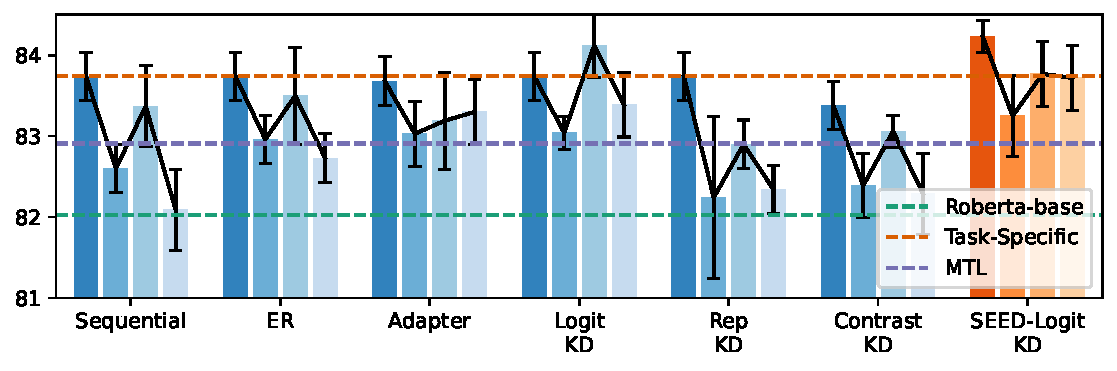
\includegraphics[width=0.48\linewidth]{acl2022/figs/academics_plots/Chemprot.pdf}}
    \subfloat[\scriptsize{RCT-Sample}]{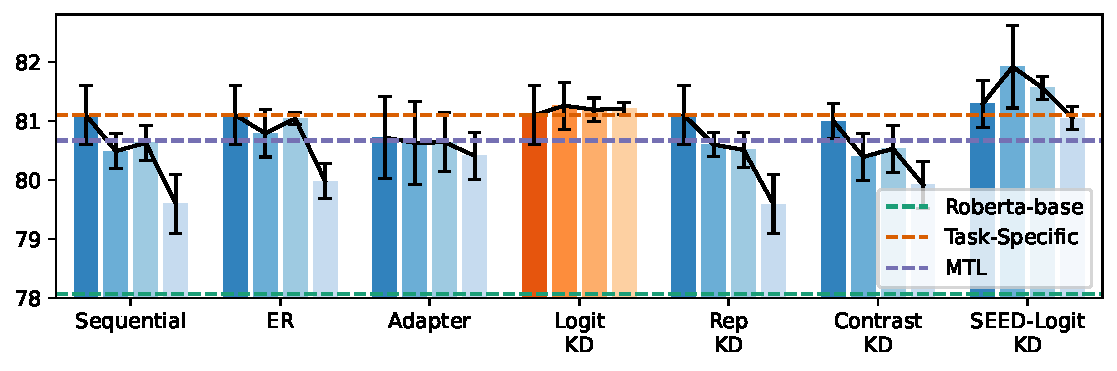
\includegraphics[width=0.48\linewidth]{acl2022/figs/academics_plots/RCT-Sample.pdf}}


    \subfloat[\scriptsize{ACL-ARC}]{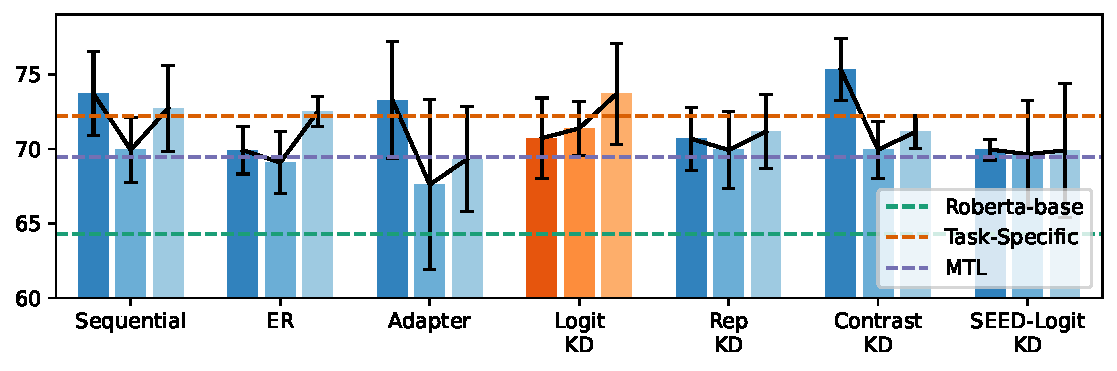
\includegraphics[width=0.48\linewidth]{acl2022/figs/academics_plots/ACL-ARC.pdf}}
    \subfloat[\scriptsize{SciERC}]{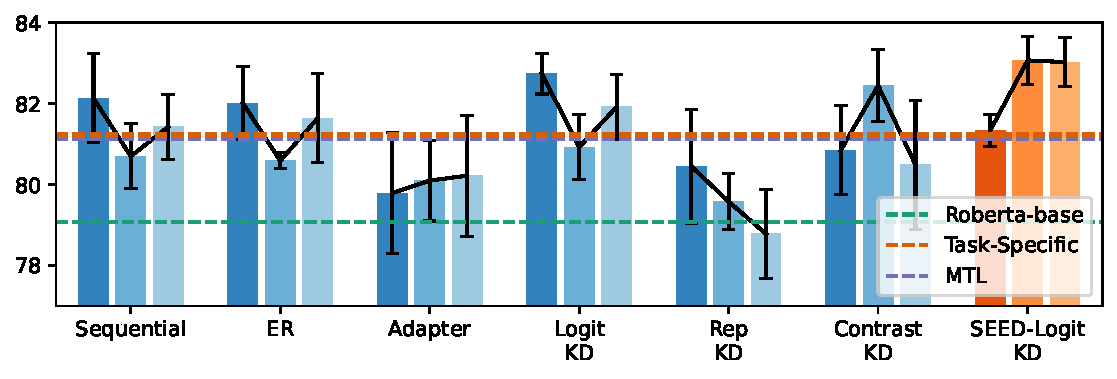
\includegraphics[width=0.48\linewidth]{acl2022/figs/academics_plots/SciERC.pdf}}
    % }
    \caption{\small \textbf{Performance evolution of downstream models.} Models are fine-tuned from checkpoints of lifelong pretrained LMs at different time steps $t$. For Chemprot and RCT-Sample from $D_1$, we use $t \in \{1,2,3,4\}$; while for ACL-ARC and SciERC from $D_2$, $t \in \{2,3,4\}$. Methods achieving the best performance at the end of training ($t=4$) is highlighted.}
    \label{fig:academics_curve}
    \vspace{-0.3cm}
\end{figure*}


\begin{figure}[]
    \centering
    % \scalebox{0.9}{
    %\subfloat[\scriptsize{Chemprot}]{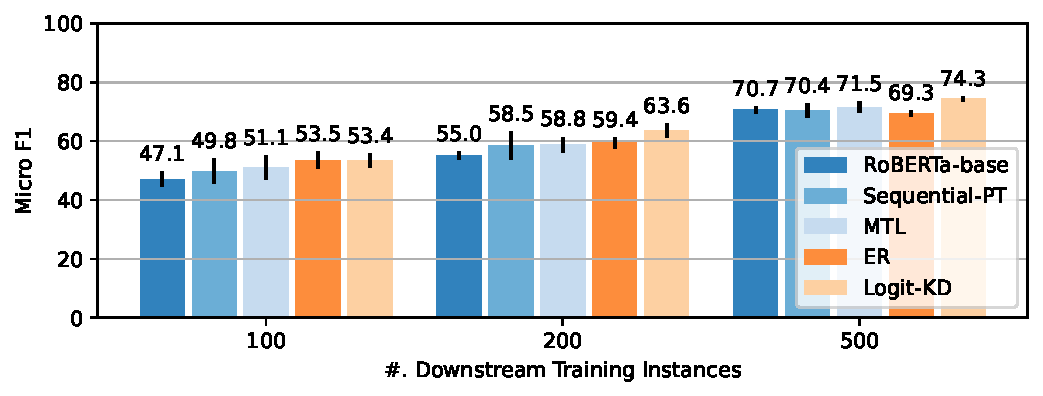
\includegraphics[width=0.94\linewidth]{acl2022/figs/academics_kshots/kshot_chemprot.pdf}}
    %\vspace{-0.3cm}
    %\subfloat[\scriptsize{RCT-Sample}]{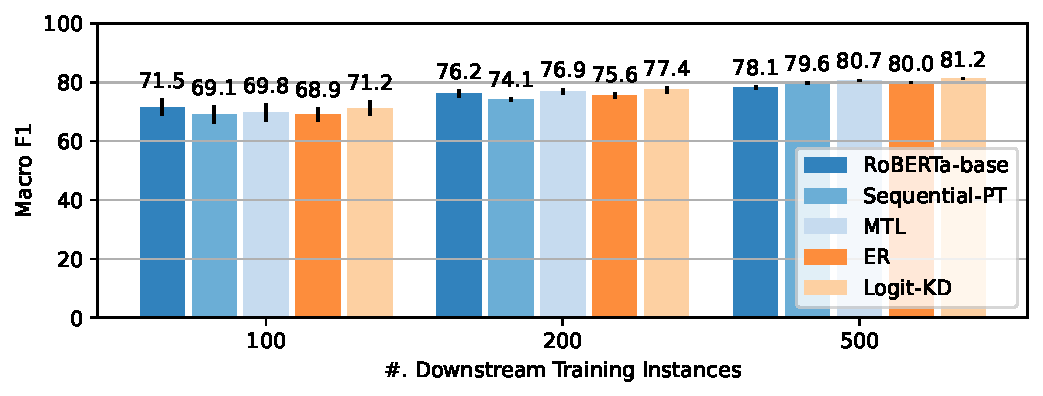
\includegraphics[width=0.94\linewidth]{acl2022/figs/academics_kshots/kshot_rct-sample.pdf}}
    %\vspace{-0.3cm}
    %\subfloat[\scriptsize{ACL-ARC}]{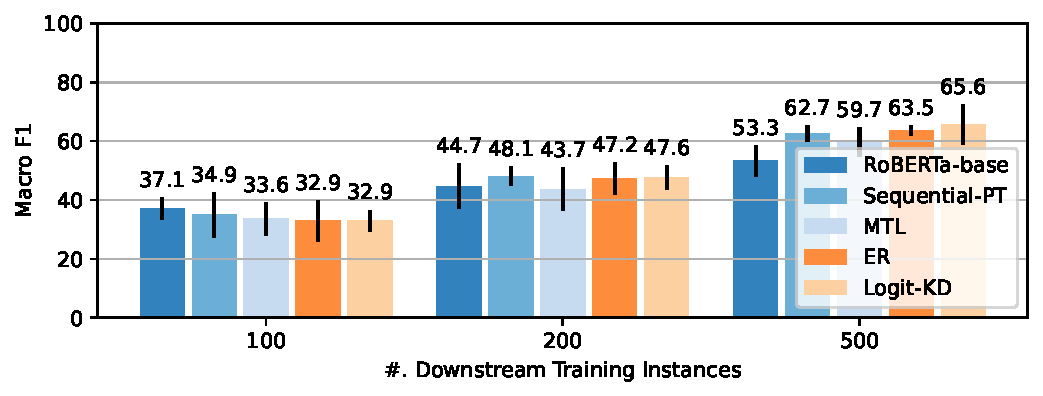
\includegraphics[width=0.94\linewidth]{acl2022/figs/academics_kshots/kshot_citation_intent.pdf}}
    % \vspace{-0.3cm}
    
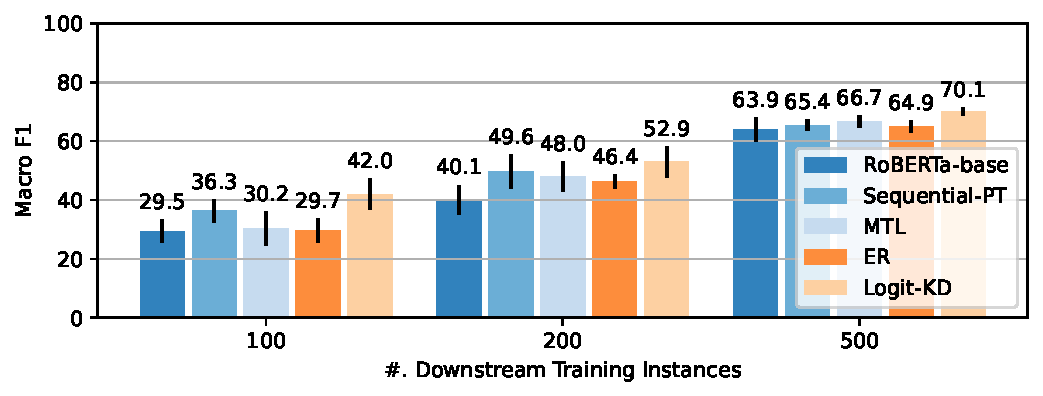
\includegraphics[width=0.98\linewidth]{acl2022/figs/academics_kshots/kshot_sciie.pdf}
    % }
    \caption{\small \textbf{Performance of downstream models with various number of training examples}, exemplified with SciERC. The models are fine-tuned from the final pretrained model ($f_4$).}
    \label{fig:academics_kshot_subset}
\end{figure}




% \paragraph{Effect of Experience Replay.} 
%\xiang{smooth out transition and recap the pros and cons of memory based methods.}
In contrast, the memory-replay based approach (ER) allows training the full parameters of the model and has been shown to be highly effective in continual learning of classification tasks~\cite{Wang2019SentenceEA, chaudhry2019tiny}. However, we surprisingly find that ER could hardly improve over Sequential Pretraining except $D_1$. % by 0.6\% and 0.4\%.
A similar pattern can be found in the MLM perplexity. 
We hypothesize that the positive effect of example replay has diminished because of the overfitting to the memory examples. Table~\ref{tab:er_tune} summarizes the effect of tuning hyperpameters in ER. When we reduce the frequency of replay (from every 10 steps to 100 steps), the MLM performance improves, which implies reduced overfitting; however, the performance of downstream task performance does not improve. When we increase the size of the memory $|M|$ from $100k$ to $10M$, the MLM perplexity also improves; still, there are still no improvements in downstream tasks. It may imply ER itself is not an effective approach for continual pretraining. %We leave more analysis into ER as future works. %We further examine the performance of ER when we experiment with a larger replay memory but notice marginal improvements, detailed in Appendix.

%\xiang{smooth out transition and recap the pros and cons of KD methods.}


Unlike ER, distillation approaches utilize richer information such as output logits or representation similarity to preserve past knowledge. We find either Logit KD or SEED-Logit KD to be most effective depending on the task, while Rep-KD and Contrastive-KD are less effective. The best performing distillation approach improves F1 over Sequential Pretraining on downstream tasks from $D_1$, $D_2$ at least by 1.0\%. However, performance on $D_3, D_4$, which come later in the data stream, does not improve over Sequential Pretraining, possibly because the distillation loss term %which tries to retain models' past knowledge 
makes the model rigid in obtaining new knowledge.

%because retaining past knowledge is a burden for obtaining new knowledge while the model has not yet suffered significantly from forgetting at the end of pretraining. 
%Still, the performance on MNER, Synthesis and Hyponym improve over the RoBERTa-base model. 
%Other distillation algorithms, such as Rep-Distill and Contrast-Distill, were not as effective as Logit-Distillation or SEED-Distillation. %However, from the performance evolution of downstream models at different pretraining checkpoint illustrated in Figure~\ref{fig:academics_curve}, we see SEED-Logit Distill could occasionally outperform Logit-Distill (\textit{e.g.,} on RCT-Sample), but in general does not outperform Logit-Distill. It implies their can be positive effect of preserving similarity structure of representations in additional to model outputs, but the effect is highly dependent on the task. 

% \paragraph{Effect of Distillation Approaches.}
%From the performance of Logit Distillation, Representation Distillation, and Contrastive Distillation, we find that only Logit Distillation could clearly reduce masked language modeling perplexity over the baselines. Representation and Contrastive Distillation do not reduce masked language modeling perplexity, which is understandable, because these two algorithms directly operate over the sentence representations, leaving the masked language model prediction head unregularized. However, we further find that only Logit distillation could consistently improve downstream task performance over Sequential Pretraining on downstream tasks in earlier domains when evaluated at the end of pretraining. The results indicate that Logit Distillation is a highly effective algorithm, and also implies that input logits are useful dark knowledge for knowledge preservation. We note the current results do not necessarily imply that the stability of representations and representational similarity is irrelevant to alleviating forgetting. In future works, we may further improve the loss term of distillation applied in Representation and Contrastive distillation.

%\xiang{Addition Analysis/discussion on ER: show the performance trend of ER wrt the size of memory, and convince people that to get little performance improvement it requires a lot larger memory, and thus less data efficient as compared to the KD methods.}

\begin{table*}[]
\centering
\scalebox{0.70}{
\begin{tabular}{@{}lccccc@{}}
\toprule
Method                                     & \#. of Forward & \#. of Backward & \#. Total   & \#. Total ($k$=10) & \ Wall Time$_{4k}$ \\ \midrule
\textit{Main results}                      &                          &                            &            &      &     \\
Sequential PT                              & $b$                      & $b$                        & $2b$       & $2b$   &  $4.0\times 10^4$ sec.  \\
ER                                         & $(1+1/k)b$               & $(1+1/k)b$                 & $(2+2/k)b$ & $2.2b$ & $4.2\times 10^4$ sec.  \\
Logit-Distill                              & $(2+2/k)b$               & $(1+1/k)b$                 & $(3+3/k)b$ & $3.3b$ &  $6.9\times 10^4$ sec.  \\
SEED-Logit-Distill                         & $(3+3/k)b$               & $(2+2/k)b$                 & $(5+5/k)b$ & $5.5b$  & $9.7\times 10^4$ sec.\\
\midrule
\textit{Additional Controlled Experiments} &                          &                            &            &        &  \\
Sequential PT$_{b^\prime=1.2b}$                     & $1.2b$                   & $1.2b$                     & $2.4b$     & $2.4b$  &  $4.4 \times 10^4$ sec. \\
%Sequential PT$_{b^\prime=1.65b}$                     & $1.65b$                   & $1.65b$                     & $3.3b$     & $3.3b$  &   \\
ER$_{k=5}$   & $1.2b$                   & $1.2b$                     & $2.4b$     & $2.4b$  &  $4.4 \times 10^4$ sec.  \\
Sparse Logit-KD                            & $1.3b$                  & $1.1b$                    & $2.4b$     & $2.4b$  & $4.4 \times 10^4$ sec.  \\
Sparse SEED-Logit-KD$_{\backslash contrast}$         & $1.3b$                  & $1.1b$                    & $2.4b$     & $2.4b$  &  $4.8 \times 10^4$ sec. \\ \bottomrule
\end{tabular}
}
\caption{Number of forward and backward passes over PTLMs and wall clock time of different approaches. The number of forward and backwards passes are computed over visits of $b$ batches from the training data stream, where $k$ is the frequency of replay. The wall clock time is calculated over 4$k$ steps of training (which is the number of training steps of a single domain in the Research Paper stream) excluding the first domain, as no replay or distillation happens while learning the first domain. In the additional controlled experiments (described in~Appendix.~\ref{apdx:controlled_computation_costs}), we control the total number of forward and backward passes of different approaches. %This also yields approximately the same wall clock time for approaches.
}
\label{tab:forward_backward_count}
\end{table*}






\paragraph{\textit{What is the gap between lifelong pretraining and multi-task learning across all the domains?}
%This needs comparison with multi-task pretraining baseline --- If we can do CL pretraining well, can CL be comparable to multi-corpus pretraining. If so, we can do CL which is much cheaper than MTL.
}
%\xiang{first say a bit on the motivation and hypothesis behind this analysis.}
Multi-Task Learning refers to the offline training paradigm, which retrain PTLMs over all corpora ($D_{1..t}$) each time a new corpus $D_t$ becomes available. 
%The practice is computationally expensive if new corpora keep emerging. 
We examine whether lifelong pretraining is comparable to multi-task pretraining in terms of performance. From Table~\ref{tab:academics} and Figure~\ref{fig:academics_curve}, we see Sequential Pretraining in general underperforms MTL except for the final domain. However, certain CL approaches, such as Logit-Distillation, could improve over MTL on all downstream tasks from the first and the second domain. We speculate the reason is that continual learning naturally provides a curriculum~\cite{Xu2020CurriculumLF, Shi2015RecurrentNN} to models where each individual task is easier to learn. 
%, in contrast to MTL, where data is mixed from multiple domains. 
The results have a positive implication that lifelong pretraining is not only more computationally efficient and requires less storage of past data, but may also improve the performance of pretraining.



\paragraph{\textit{Does lifelong pretraining make models more data efficient?}}
In Table~\ref{fig:academics_kshot_subset}, we further examine the performance of final pretrained models under different amounts of training examples. We include full results in Appendix~\ref{apdx:low_resource}. We find in general, performance improvements are more significant in the low-resource setup. %\xiang{revise and expand a bit more on the msgs.}
%We hypothesize it is because the accumulated knowledge over continual pretraining creates a better model initialization to help learn downstream tasks in a more data-efficient manner.



\paragraph{\textit{Computational Costs.}} We quantify computational costs of different CL algorithms with the number of forward and backward passes in Table~\ref{tab:forward_backward_count} and present additional experiments with controlled computational costs in Appendix~\ref{apdx:controlled_computation_costs}. We find additional computational cost is necessary for performance improvement of distillation-based CL. However, it is not possible to trade performance simply by investing more computation budget with arbitrary CL algorithms. We leave detailed discussions in Appendix~\ref{apdx:controlled_computation_costs}.

%Exp 2 Setup (fine-tuning data efficiency): take checkpoints from (original LM, task-specific LM, CL-LM); do fine-tuning and track the performance wrt fine-tuning steps.
%}







\subsection{Temporal Data Stream}
\label{ssec:temporal_data_stream}

We conduct analysis on pretraining PTLM on chronologically-ordered tweet corpora, to understand whether lifelong pretraining helps adaptation to the latest data and improves temporal generalization ability. %In this setup, the pretrained corpora $D_{1..4}$ are tweet data in different years%and the pretrained LMs are fine-tuned on Hashtag and Emoji prediction data from each year of $D_{1..4}$.
% We then move our focus to the next set of research questions regarding whether lifelong pretraining improves model's adaptation to latest data and temporal generalization when the data stream is chronologically ordered.
%\xiang{add 1-2 sentences on overview of the exp setup?}
%We study a series of research questions using the tweet stream. 
The results are summarized in Table~\ref{tab:twitter}.
% We summarize our findings below.

%\xiang{\paragraph{\textit{Q1: Will LM be outdated?}}
%updated LM vs. original LM
%}
\paragraph{\textit{Will LMs be outdated?}} %We first examine whether the LM pretrained specifically on the tweets of 2014 (the row of Task-Specific (2014) in Table~\ref{tab:twitter}) becomes less effective when applied to downstream datasets from subsequent years. 
We compare the performance of Task-Specific (2014) to the Task-Specific models pretrained on the year of downstream datasets (noted as Task-Specific (Latest)) and notice consistent improvements in downstream tasks in 2018 and 2020  (first two columns in Table~\ref{tab:twitter}). Sequential Pretraining could also outperform the Task-Specific (2014) model. It verifies that language models may get outdated over time, but the issue can be addressed by task-specific or lifelong pretraining over the latest corpora.

% As we mentioned in Sec.~\ref{ssec:evaluation_protocols}, over chronologically ordered data streams, the performance over the latest data is of higher importance. Therefore, in Table~\ref{tab:twitter}, we focus on the hashtag prediction performance in the year 2020. Unfortunately, we find continually pretrained models do not improve over task-specific models, which are only pretrained over the latest year. It may imply knowledge from earlier years is redundant for the hashtag prediction task given the latest data. 

\begin{table}[]
\centering
\scalebox{0.607}{
% Please add the following required packages to your document preamble:
% \usepackage{booktabs}
\begin{tabular}{@{}lcccc@{}}
\toprule
Years                  & 2018 $(D_3)$              & 2020 $(D_4)$              & \begin{tabular}[c]{@{}c@{}}2014 $(D_1)$ \\ $\to$ 2020 $(D_4)$\end{tabular} & \begin{tabular}[c]{@{}c@{}}2016 $(D_2)$\\ $\to$ 2020 $(D_4)$\end{tabular} \\ \midrule
\multicolumn{5}{c}{Hashtag Prediction}                                                                   \\ \midrule
RoBERTa-base           & 48.08$_{\pm 1.0}$ & 56.42$_{\pm 0.2}$  & 39.31$_{\pm 2.7}$ & 42.23$_{\pm 2.7}$ \\
Sequential PT          & 56.79$_{\pm 0.5}$ & 59.85$_{\pm 0.4}$  & 44.00$_{\pm 1.1}$ & 49.87$_{\pm 1.8}$ \\
ER                     & 56.93$_{\pm 0.1}$ & 59.56$_{\pm 1.7}$  & 43.31$_{\pm 0.2}$ & 50.72$_{\pm 0.6}$ \\
%Adapter                & 54.34$_{\pm1.7}$  & 59.01$_{\pm 1.0 }$ & 42.61$_{\pm 0.5}$ & 48.00$_{\pm 1.6}$ \\
Logit-KD               & \textbf{58.21$_{\pm 0.5}$} & 60.52$_{\pm 0.2}$  & 44.26$_{\pm 0.9}$ & 50.92$_{\pm 0.8}$ \\
%Rep-KD                 & 55.79$_{\pm 1.4}$ & 59.80$_{\pm 0.2}$  & 42.48$_{\pm 0.2}$ & 50.38$_{\pm 1.5}$ \\
Contrast-KD            & 57.94$_{\pm 0.4}$ & 59.54$_{\pm 0.3}$  & 45.22$_{\pm 0.1}$ & \textbf{52.14$_{\pm 1.1}$} \\
SEED-KD                & 56.87$_{\pm 0.2}$ & 59.71$_{\pm 0.2}$  & 43.39$_{\pm 0.4}$ & 49.62$_{\pm 1.0}$ \\
SEED-Logit-KD          & 57.75$_{\pm 0.4}$ & \textbf{60.74$_{\pm 0.6}$}  & \textbf{45.35$_{\pm 0.6}$} & 51.56$_{\pm 0.7}$ \\  \midrule
Task-Specific (2014)   & 56.16$_{\pm 0.6}$ & 59.59$_{\pm 0.3}$  & 44.34$_{\pm 0.6}$ & 49.26$_{\pm 0.7}$ \\
Task-Specific (Latest) & 56.61$_{\pm 0.4}$ & 59.87$_{\pm 0.6}$  & 43.44$_{\pm 0.5}$ & 49.41$_{\pm 1.1}$ \\
MTL                    & 57.89$_{\pm 0.4}$ & 59.95$_{\pm 0.3}$  & 44.04$_{\pm 0.3}$ & 50.37$_{\pm 0.3}$ \\
\midrule
\multicolumn{5}{c}{Emoji Prediction}                                                                     \\ \midrule
RoBERTa-base           & 25.71$_{\pm 0.1}$ & 24.42$_{\pm 0.2}$  & 12.02$_{\pm 0.4}$ & 13.24$_{\pm 0.2}$ \\
Sequential PT          & 29.30$_{\pm 0.1}$ & 27.69$_{\pm 0.1}$  & 14.20$_{\pm 0.2}$ & 16.08$_{\pm 1.4}$ \\
ER                     & 29.50$_{\pm 0.1}$ & 27.75$_{\pm 0.1}$  & 14.36$_{\pm 0.4}$ & 16.82$_{\pm 0.3}$ \\
%Adapter                & 28.72$_{\pm 0.0}$ & 26.80$_{\pm 0.3}$  & 13.53$_{\pm 0.2}$ & 15.68$_{\pm 0.3}$ \\
Logit-KD               & 29.77$_{\pm 0.1}$ & 27.80$_{\pm 0.1}$  & 14.20$_{\pm 0.3}$ & 16.28$_{\pm 1.1}$ \\
%Rep-KD                 & 29.45$_{\pm 0.1}$ & 27.27$_{\pm 0.2}$  & 13.89$_{\pm 0.1}$ & 16.03$_{\pm 0.3}$ \\
Contrast-KD            & 29.48$_{\pm 0.2}$ & 27.72$_{\pm 0.3}$  & \textbf{14.42$_{\pm 0.3}$} & \textbf{17.52$_{\pm 0.1}$} \\
SEED-KD                & \textbf{30.12$_{\pm 0.1}$} & 27.66$_{\pm 0.1}$  & 14.36$_{\pm 0.1}$ & 16.97$_{\pm 0.4}$ \\
SEED-Logit-KD          & 29.98$_{\pm 0.1}$ & \textbf{27.84$_{\pm 0.2}$}  & 14.36$_{\pm 0.1}$ & 16.97$_{\pm 0.3}$ \\ \midrule
Task-Specific (2014)   & 28.94$_{\pm 0.0}$ & 26.98$_{\pm 0.2}$  & 13.39$_{\pm 0.2}$ & 15.14$_{\pm 0.2}$ \\
Task-Specific (Latest) & 29.06$_{\pm 0.2}$ & 27.19$_{\pm 0.1}$  & 13.00$_{\pm 0.2}$ & 14.48$_{\pm 0.3}$ \\
MTL                    & 29.52$_{\pm 0.2}$ & 27.47$_{\pm 0.0}$  & 14.07$_{\pm 0.2}$ & 16.64$_{\pm0.2}$   \\  \bottomrule
\end{tabular}
}
\caption{\small \textbf{Results on temporal data stream.} We show fine-tuning performance over years 2018 and 2020 ($D_3$, $D_4$) and the Temporal generalization from 2014 or 2016 to 2020 data ($D_1\to D_4$, $D_2 \to D_4$) on Twitter Hashtag and Emoji prediction datasets. Models are fine-tuned from the final pre-trained model $f_T$. We include full results on other years ($D_1$, $D_2$, $D_3 \to D_4$) in Appendix~\ref{apdx:full_tweet_results}.
%\texttt{Year 1}$\to$\texttt{Year 2} indicates the hashtag prediction model is fine-tuned on data in year \texttt{Year 1}, and evaluated on test data in \texttt{Year 2}.
}
\label{tab:twitter}
\end{table}



\paragraph{\textit{Does lifelong pretraining help improve the downstream model’s performance on latest data?}}
%\xiang{1) Where (what part of results) to look for the observations? (do we look for year 2020, or all years, or sth else?)
%2) What is the main takeaway distilled in an accessible sentence? Can we have that up front?
%}
We show that downstream model's performance over later data ($D_3, D_4$) can be improved over Task-Specific models when continual learning algorithms are applied. From the first two columns of Table~\ref{tab:twitter}, %we see no consistent improvement of simple Sequential Pretraining over Task-Specific models in 2018 and 2020 ($D_3, D_4$).  %in hashtag prediction tasks, it achieves 0.18 higher score over data of year 2018, but achieves 0.02 lower score over data of year 2020. 
%We find continual learning algorithms could improve the performance by a small degree. 
we see Logit-KD and SEED-KD improve Hashtag prediction score over data of years 2018 and 2020. %by 1.60 and 0.65 respectively over Sequentail PT. %, and improves emoji prediction F1 by 0.71 and 0.61 over Task-Specific models. 
SEED-Logit KD further improves prediction F1 on Emoji prediction. 
Note that these findings are in contrast to the research paper stream, where CL algorithms do not improve performance in the latest domain $D_4$. The reason can be the higher similarity between domains in the tweet corpora making the knowledge transfer easier, which is further discussed in Appendix~\ref{apdx:analysis_data_streams}.

\paragraph{\textit{Does lifelong pretraining improve temporal generalization?}} 
%\xiang{Some brief re-cap on motivation of this ability; the exp setting; and eval protocol.}
Temporal generalization evaluates downstream performance over latest test data when fine-tuned over outdated training data. 
%The setup is prevalent in practice for systems deployed online. 
We show lifelong pretraining brings clear improvement to temporal generalization.
From Table~\ref{tab:twitter}, we see even Sequential Pretraining could improve over the model pretrained merely on the year 2020 data (Task-Specific (2020)) consistently. We find performance further improves with CL algorithms applied. SEED-Logit-KD performs best in general on crossyear hashtag prediction tasks. %improving scores over Task-Specific (2020) by 1.75 and 2.91. 
In crossyear emoji prediction, we find Contrast-KD and SEED-KD perform best. We also find that SEED-Logit-KD could slightly outperform Logit-KD. %, improving over Task-Specific (2020) by 1.42, 2.67 and 1.60 respectively.

%In th   e further investigate whether continual learning algorithms improve temporal generalization, where the hashtags prediction models are fine-tuned on outdated training data (2014, 2016, 2018) but evaluated on the latest data (2020). From Table~\ref{tab:twitter_tg}, we see lifelong pretraining almost always improve performance over Task-Specific LM. It implies pretraining data from earlier years are helpful for temporal generalization. However, we do not find a consistent trend within the performance of different continual learning algorithms: Logit-KD$_{\text{first}}$ performs the best in 2014$\to$2020 generalization, while Sequential Pretraining performs the best in 2018$\to$2020 generalization. The mixed results encourage future works to study more effective lifelong pretraining algorithms.


%\begin{table}[]
\centering
\scalebox{0.66}{
\begin{tabular}{@{}lccc@{}}
\toprule
Task          & 2014 $\to$ 2020 & 2016 $\to$ 2020 & 2018 $\to$ 2020 \\ 
\midrule
\multicolumn{4}{c}{Crossyear Hashtag Prediction}                        \\
\midrule
RoBERTa-base  & 39.31$_{\pm 2.7}$     & 42.23$_{\pm 2.7}$     & 37.19$_{\pm 2.1}$     \\
Sequential PT       & 44.00$_{\pm 1.1}$     & 49.87$_{\pm 1.8}$     & 46.63$_{\pm 0.9}$     \\
ER            & 43.31$_{\pm 0.2}$     & 50.72$_{\pm 0.6}$     & 46.27$_{\pm 0.4}$     \\
Adapter       &    42.61$_{\pm 0.5}$           &        48.00$_{\pm 1.6}$       &   42.63$_{\pm 0.9}$            \\
Logit-KD      & 44.26$_{\pm 0.9}$     & 50.92$_{\pm 0.8}$     & 46.84$_{\pm 1.0}$     \\
Rep-KD        &     42.48$_{\pm 0.2}$      &        50.38$_{\pm 1.5}$       &       42.23$_{\pm 0.2}$        \\
Contrast-KD   &      45.22$_{\pm 0.1}$       &       52.14$_{\pm 1.1}$         &            47.47$_{\pm 0.8}$   \\
SEED-KD & 43.39$_{\pm 0.4}$  & 49.62$_{\pm 1.0}$ & 46.37$_{\pm 0.8}$ \\
SEED-Logit-KD &   45.35$_{\pm 0.6}$      &      51.56$_{\pm 0.7}$     &         47.74$_{\pm 0.3}$      \\
Task-Specific (2014) &      44.34$_{\pm 0.6}$         &         49.26$_{\pm 0.7}$      &        45.09$_{\pm 0.7}$       \\
Task-Specific (2020) &      43.44$_{\pm 0.5}$          &           49.41$_{\pm 1.1}$                &          44.34$_{\pm 0.4}$        \\
- \textit{4x steps}& 44.34$_{\pm 0.6}$     & 51.78$_{\pm 0.7}$     & 44.69$_{\pm 0.7}$     \\
MTL           & 44.04$_{\pm 0.3}$     & 50.37$_{\pm 0.3}$     & 44.31$_{\pm 0.0}$     \\ 
\midrule
\multicolumn{4}{c}{Crossyear Emoji Prediction}                          \\ \midrule
RoBERTa-base  & 12.02$_{\pm 0.4}$     & 13.24$_{\pm 0.2}$     & 18.67$_{\pm 0.1}$     \\
Sequential PT       & 14.20$_{\pm 0.2}$     & 16.08$_{\pm 1.4}$     & 21.06$_{\pm 0.9}$     \\
ER            & 14.36$_{\pm 0.4}$     & 16.82$_{\pm 0.3}$     & 21.57$_{\pm 0.1}$     \\
Adapter       &     13.53$_{\pm 0.2}$       &   15.68$_{\pm 0.3}$        &      20.64$_{\pm 0.1}$         \\
Logit-KD      & 14.20$_{\pm 0.3}$     & 16.28$_{\pm 1.1}$     & 21.29$_{\pm 1.0}$     \\
Rep-KD        &    13.89$_{\pm 0.1}$       &        16.03$_{\pm 0.3}$       &           20.86$_{\pm 0.2}$    \\
Contrast-KD   &     14.42$_{\pm 0.3}$       &       17.52$_{\pm 0.1}$        &      21.43$_{\pm 0.1}$         \\
SEED-KD & 14.36$_{\pm 0.1}$ & 16.97$_{\pm 0.4}$ & 21.88$_{\pm 0.3}$ \\
SEED-Logit-KD & 14.36$_{\pm 0.1}$    &     16.97$_{\pm 0.3}$      &         21.62$_{\pm 0.1}$      \\
Task-Specific (2014) &    13.39$_{\pm 0.2}$        &        15.14$_{\pm 0.2}$                   &       20.79$_{\pm 0.3}$              \\
Task-Specific (2020) & 13.00$_{\pm 0.2}$     & 14.48$_{\pm 0.3}$     & 19.30$_{\pm 0.2}$     \\
- \textit{4x steps}& 12.90$_{\pm 0.4}$     & 14.85$_{\pm 0.3}$     & 19.83$_{\pm 0.2}$     \\
MTL           &     14.07$_{\pm 0.2}$       &       16.64$_{\pm0.2}$    &       20.94$_{\pm 0.7}$   \\ 
\bottomrule
\end{tabular}
}
\caption{\small Temporal generalization performance on Twitter Hashtag prediction datasets fine-tuned from the final pre-trained model. \texttt{Year 1}$\to$\texttt{Year 2} indicates the hashtag prediction model is fine-tuned on data in year \texttt{Year 1}, and evaluated on test data in \texttt{Year 2}.}
\vspace{-0.3cm}
\label{tab:twitter_tg_full}
\end{table}


%\subsection{Performance of Existing Continual Learning Algorithms}
%For memory based approaches, we are able to quantify the benefit of continual learning algorithms by comparing their performance to Sequential Pretraining, which shares the same model architecture but does not apply any continual learning algorithms. We notice that ER could improve performance on three of the four datasets. 

%Adapter-based methods do not suffer from forgetting, and is able to improve over Roberta-base and Adapter-Fresh models that are not trained over academic corpora. However, we notice the performance of the best-performing adapter methods (Adapter-Single) is only on par with ER, despite perfect mitigation of forgetting. We also tried fusing information from multiple (2 or 4, which correspond to Adapter-Fusion$_2$ and Adapter-Fusion$_4$), but the performance did not improvement. We also experimented with a larger hidden dimension within the adapters (Adapter-Large), while the performance increased only marginally. We hypothesize that the modeling capacity of adapter models is the bottleneck of the performance. 



% \subsection{Performance of Contrastive Learning Experience Replay}
% We compare our proposed CER approach with ER. We notice CER could improve performance over all datasets compared to ER. We further show the performance improvement originates from that CER could reduce catastrophic forgetting, rather than the side effect of adding the contrastive learning that allows learning better representation: by comparing Single and Single-Contrast, we see the improvement is not clear by adding the contrastive learning term in the single-task learning case.


\section{Related Works}
\vspace{-0.1cm}
%\xiang{compress to ~1.1 page}

\paragraph{Domain and Temporal Adaptation of Language Models.} 
~\citet{Gururangan2020DontSP} study adaptation of PTLMs to domain-specific corpora. ~\citet{Arumae2020AnEI} study algorithms to mitigate forgetting in original PTLMs, but does not investigate forgetting that happens over a sequence of domains. \citet{Maronikolakis2021MultidomainPL,Rttger2021TemporalAO, luu2021time} proposes sequential pretraining over domains or emerging data, but did not investigate CL algorithms. Several recent studies have demonstrated the necessity of adapting LMs over time~\cite{Lazaridou2021PitfallsOS} while %some of them 
specifically focusing on factual knowledge~\cite{Dhingra2021TimeAwareLM, jang2021towards}.

\paragraph{Continual Learning Algorithms in NLP.}
Continual learning in NLP has mainly been studied for classification tasks. An effective approach is to utilize a number of stored past examples~\cite{dAutume2019EpisodicMI,Wang2020EfficientML}, or pseudo examples (\textit{e.g.,} the ones generated with a PTLM~\cite{Sun2020LAMOLLM,Kanwatchara2021RationalLA}). Recent extensions of the algorithm~\cite{Chuang2020LifelongLK} perform knowledge distillation with generated pseudo examples. Other lines of works focus on regularization over the sentence representations~\cite{Wang2019SentenceEA,Huang2021ContinualLF,Liu2019ContinualLF} or directly merging models in the parameter space~\cite{Matena2021MergingMW}. % propose an information disentanglement and regularization-based approach which disentangles and applies separate regularization to task-agnostic and task-specific representations.
%In addition, methods such as EWC~\cite{Schwarz2018ProgressC} and online EWC~\cite{Kirkpatrick2017OvercomingCF} performs regularization directly in the weight space. The algorithms are not intensively studied for NLP tasks. M
Model expansion-based approaches~\cite{Liu2019ContinualLF,Pfeiffer2021AdapterFusionNT}, including learning domain specific expert models~\cite{Gururangan2021DEMixLD}, are also actively studied.~\citet{wu2022pretrained} present a comparative study of algorithms in the context of continual fine-tuning over NLP tasks.






\section{Conclusion}
\vspace{-0.1cm}
In this paper, we formulated the lifelong language model pretraining problem and constructed two data streams associated with downstream datasets. 
%We constructed the domain-incremental research paper stream and the chronologically-ordered tweet stream, each of which is representative of a practical scenario of continual pretraining. 
We evaluated knowledge retention, adaptation to the latest data, and temporal generalization ability of continually pretrained language models. 
%We evaluated a number of continual learning algorithms spanning over adapters, memory replay, and distillation-based approaches. 
Our experiments show distillation-based approaches being most effective in these evaluation setups. A limitation of the work is that it has not been fully addressed whether there exists a variant of distillation-based CL approach that consistently outperforms Logit-KD. Based on the current observation, we conclude the performance of different KD approaches for CL is highly task-dependent.
%Over the tweet stream, we find continual pretraining improves adaptation ability to the latest data and temporal generalization. 
It asks for more future works into continual learning algorithms within the proposed problem setup.


%In our setup, the model is continuously pretrained over a sequence of unlabeled corpus and is fine-tuend over downstream tasks related to pretraining. We evaluate the performance of various continual learning algorithms, encompassing adapter based, memory based, and distillation based approaches. We proposed a novel continual learning algorithm, contrastive learning experience replay (CER) to improve the informativeness of the replay memory and effectively mitigate forgetting in the representation space. Our experiments over academic paper datasets show CER is efficient in reducing catastrohpic forgetting. We will further perform experiments over other datasets proposed in the paper and include more continual learning baselines for study.



\bibliography{main}
\bibliographystyle{acl_natbib}

\appendix
\clearpage
\newpage

\section{Detailed Experiment Settings}
\label{sec:hyps}
We use a linearly decreasing learning rate initialized with 5e-4 on the research paper stream and 3e-4 on the tweet stream. On the research paper stream, we train the model for 8,000 steps in the first task, and 4,000 steps in the subsequent tasks. On the tweet stream, we train the model for 8,000 steps in all tasks. We hold out 128,000 sentences from each corpus to evaluate MLM performance. As the size of pretraining corpora is large, during training, each training example is visited only once. We use the masked language modeling perplexity over held-out validation sets of the pretraining corpora as the metrics for hyperparameter tuning. 
Common hyperparameters such as learning rate and batch sizes are tuned with Task-specific models with the first task. Hyperparameters that are specific to continual learning algorithms, such as the scale of the distillation loss, is tuned using the first two domains in the stream according to the MLM performance over validation sets. The weight of the distillation term $\alpha$ is set as 1.0 for logit distillation and 0.1 for other distillation algorithms. By default, we replay or perform distillation with a mini-batch of examples from the replay memory every 10 training steps in ER and Distillation-based CL approaches. We use the huggingface transformers library \url{https://github.com/huggingface/transformers} for implementation.
%\xiang{1-2 sentences on how hps of all the methods are determined; what metrics/loss we looked at.}
%In contrastive distillation approaches, we set $\alpha$=1 and $\tau$=0.05.

%Note that the label space of hashtag prediction can be different between years. In our experiments, for evaluation of temporal generalization, we use the label set of the earlier year, and collect examples from the held-out 1M tweets in the latest year that have at least one of the hashtags in the earlier year. We sub-sample 10,000 examples as the test set.



\section{Low-Resource Fine-Tuning}
\label{apdx:low_resource}


%xiang{\paragraph{\textit{Q5: Will continually pretrained model adapt faster to a new domain?}}
%--> pretraining data efficiency comparison between a continually pretrained model vs. roberta, when further pretrained to a new domain
%}
\begin{figure}[]
    \centering
    % \scalebox{0.9}{
    \subfloat[\scriptsize{Chemprot}]{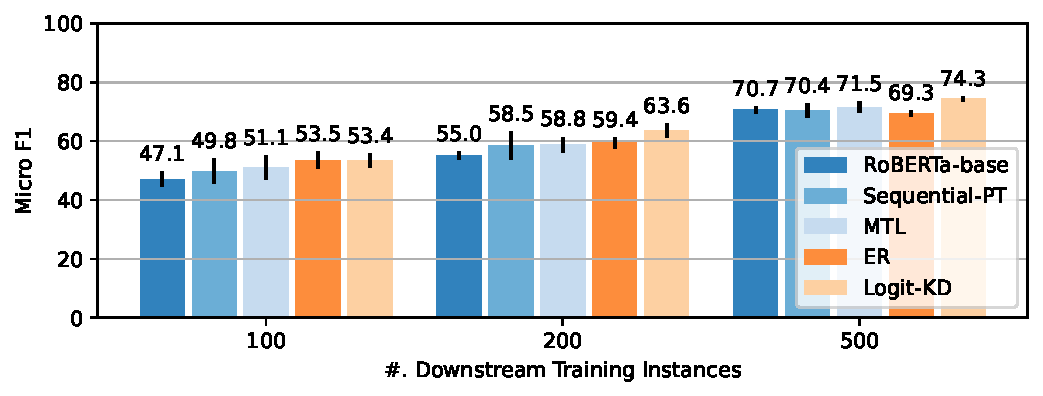
\includegraphics[width=0.94\linewidth]{acl2022/figs/academics_kshots/kshot_chemprot.pdf}}
    
    %\subfloat[\scriptsize{RCT-Sample}]{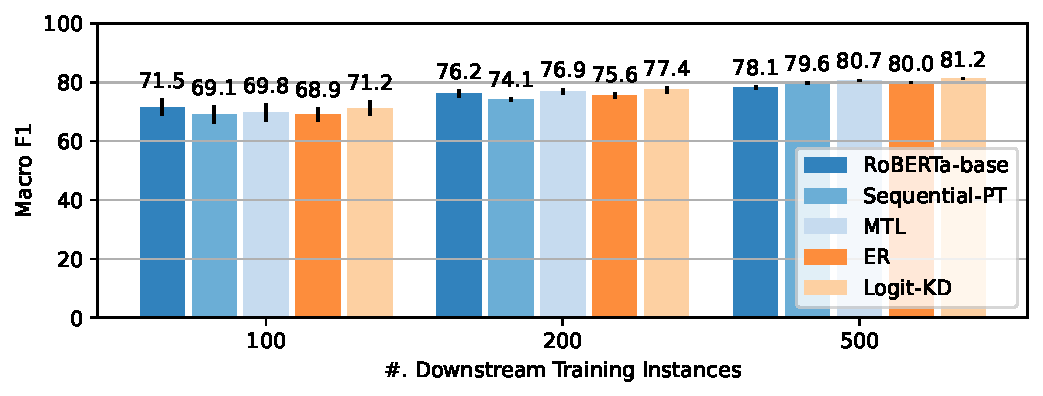
\includegraphics[width=0.94\linewidth]{acl2022/figs/academics_kshots/kshot_rct-sample.pdf}}
    
    %\vspace{-0.3cm}
    %\subfloat[\scriptsize{ACL-ARC}]{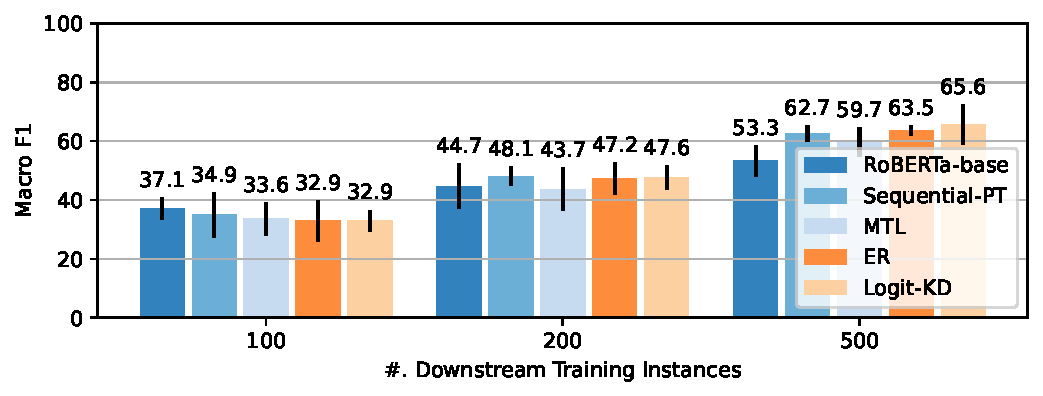
\includegraphics[width=0.94\linewidth]{acl2022/figs/academics_kshots/kshot_citation_intent.pdf}}
    % \vspace{-0.3cm}
    
    \subfloat[\scriptsize{SciERC}]{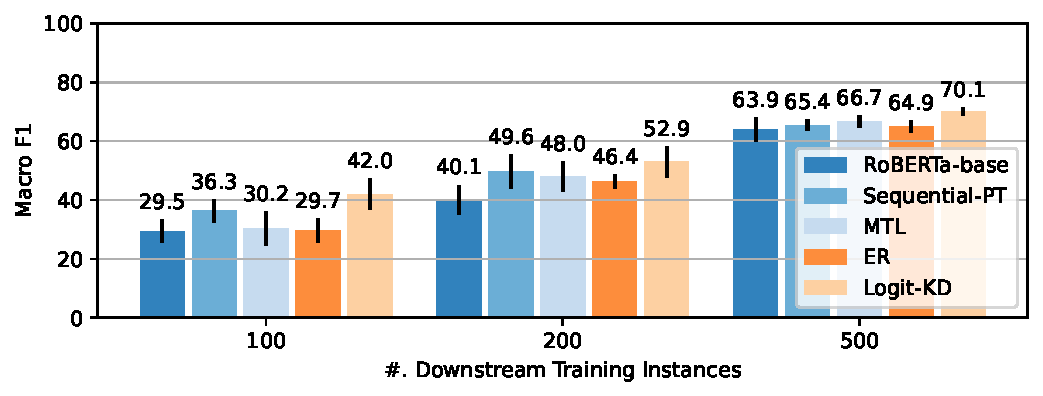
\includegraphics[width=0.94\linewidth]{acl2022/figs/academics_kshots/kshot_sciie.pdf}}
    % }
    \caption{\small Performance of downstream models with various number of training examples. The models are fine-tuned from the final pretrained model ($f_4$).}
    \label{fig:academics_kshot}
\end{figure}

Figure~\ref{fig:academics_kshot} summarizes the performance of fine-tuned models from the final model checkpoint ($t=4$) using different amount of downstream training examples. We see on Chemprot and SciERC, the benefit of Sequential Pretraining over RoBERTa-base is more significant in low-resource fine-tuning setups. 
%while on RCT-Sample and ACL-ARC, Sequential Pretraining improves over RoBERTa-base when there are sufficient amount of training examples. 
Whenever Seqential Pretraining outperforms RoBERTa-base, we notice Logit-KD could further improve over Sequential Pretraining.

\section{Full Results over the Tweet Stream}
\label{apdx:full_tweet_results}
\begin{table}[]
\centering
\scalebox{0.66}{
\begin{tabular}{@{}lcccc@{}}
\toprule
Task          & 2014                 & 2016                 & 2018                 & 2020                 \\ \midrule
\multicolumn{5}{c}{Hashtag Prediction}                                                      \\ \midrule
RoBERTa-base  & 56.65$_{\pm 0.6}$            & 45.50$_{\pm 2.1}$            & 48.08$_{\pm 1.0}$            & 56.42$_{\pm 0.2}$            \\
Sequential PT        & 59.00$_{\pm 0.1}$            & 54.28$_{\pm 0.3}$            & 56.79$_{\pm 0.5}$            & 59.85$_{\pm 0.4}$            \\
ER            & 59.00$_{\pm 0.1}$            & 54.90$_{\pm 0.2}$            & 56.93$_{\pm 0.1}$            & 59.56$_{\pm 1.7}$            \\
Adapter       &     58.76$_{\pm 0.7}$         &         52.55$_{\pm 1.5}$             &           54.34$_{\pm1.7}$           &          59.01$_{\pm 1.0 }$            \\
Logit-KD      &   60.93$_{\pm 0.5}$        &        55.96$_{\pm 0.2}$              &            58.21$_{\pm 0.5}$          &        60.52$_{\pm 0.2}$              \\
Rep-KD        &      60.47$_{\pm 0.1}$           &      51.77$_{\pm 2.6}$                &              55.79$_{\pm 1.4}$        &          59.80$_{\pm 0.2}$ \\
Contrast-KD   &       60.72$_{\pm 0.6}$         &      55.85$_{\pm 0.0}$              &         57.94$_{\pm 0.4}$         &     59.54$_{\pm 0.3}$                 \\
SEED-KD & 58.82$_{\pm 0.4}$ & 54.55$_{\pm 0.5}$ & 56.87$_{\pm 0.2}$ & 59.71$_{\pm 0.2}$ \\
SEED-Logit-KD &        61.28$_{\pm 0.2}$           &            55.59$_{\pm 0.5}$          &                57.75$_{\pm 0.4}$      &          60.74$_{\pm 0.6}$            \\
Task-Specific (2014) & 61.62$_{\pm 0.3}$            & 55.38$_{\pm 0.6}$            & 56.16$_{\pm 0.6}$            & 59.59$_{\pm 0.3}$            \\
Task-Specific (Latest) & 59.91$_{\pm 0.3}$            & 55.47$_{\pm 1.0}$            & 56.61$_{\pm 0.4}$            & 59.87$_{\pm 0.6}$            \\
MTL           & 60.51$_{\pm 0.3}$            & 55.16$_{\pm 1.6}$            & 57.89$_{\pm 0.4}$            & 59.95$_{\pm 0.3}$            \\ \midrule
               \multicolumn{5}{c}{Emoji Prediction}                                                      \\ \midrule
RoBERTa-base  & 28.73$_{\pm 0.2}$            & 26.86$_{\pm 0.2}$            & 25.71$_{\pm 0.1}$            & 24.42$_{\pm 0.2}$            \\
Sequential PT       & 32.69$_{\pm 0.2}$            & 30.55$_{\pm 0.3}$            & 29.30$_{\pm 0.1}$            & 27.69$_{\pm 0.1}$            \\
ER            & 32.88$_{\pm 0.2}$            & 30.52$_{\pm 0.2}$            & 29.50$_{\pm 0.1}$            & 27.75$_{\pm 0.1}$            \\
Adapter       &      32.15$_{\pm 0.2}$         &        29.85$_{\pm 0.0}$         &            28.72$_{\pm 0.0}$          &     26.80$_{\pm 0.3}$             \\
Logit-KD      & 33.08$_{\pm 0.3}$            & 30.88$_{\pm 0.1}$            & 29.77$_{\pm 0.1}$            & 27.80$_{\pm 0.1}$            \\
Rep-KD        &      32.71$_{\pm 0.2}$         &        30.51$_{\pm 0.2}$              &        29.45$_{\pm 0.1}$          &        27.27$_{\pm 0.2}$          \\
Contrast-KD   & 32.90$_{\pm 0.1}$            & 31.01$_{\pm 0.1}$            & 29.48$_{\pm 0.2}$            & 27.72$_{\pm 0.3}$            \\
SEED-KD & 32.91$_{\pm 0.1}$ & 30.84$_{\pm 0.3}$ & 30.12$_{\pm 0.1}$ & 27.66$_{\pm 0.1}$ \\
SEED-Logit-KD &      33.28$_{\pm 0.1}$          &      31.17$_{\pm 0.1}$                &           29.98$_{\pm 0.1}$       &       27.84$_{\pm 0.2}$               \\
Task-Specific (2014) & 33.37$_{\pm 0.2}$            & 30.54$_{\pm 0.3}$            & 28.94$_{\pm 0.0}$            & 26.98$_{\pm 0.2}$            \\
Task-Specific (Latest) & 32.31$_{\pm 0.0}$            & 29.83$_{\pm 0.5}$            & 29.06$_{\pm 0.2}$            & 27.19$_{\pm 0.1}$            \\
MTL           &  32.78$_{\pm 0.1}$  & 30.54$_{\pm 0.0}$ & 29.52$_{\pm 0.2}$ &  27.47$_{\pm 0.0}$ \\  \bottomrule
\end{tabular}
}
\caption{\small Full performance on Twitter Hashtag prediction and Emoji prediction, fine-tuned from the pre-trained model in the final time step.}
\label{tab:twitter_full}
\end{table}



% \begin{table}[]
% \centering
% \scalebox{0.72}{
% \begin{tabular}{@{}lcccc@{}}
% \toprule
%           \textbf{Tweet year}  & \textbf{2014}      & \textbf{2016}      & \textbf{2018}      & \textbf{2020}      \\ \midrule
% Roberta-base & 56.65$_{\pm 0.6}$ & 45.50$_{\pm 2.1}$ & 48.08$_{\pm 1.0}$ & 56.42$_{\pm 0.2}$ \\
% Naive CL     & 59.00$_{\pm 0.1}$ & 54.28$_{\pm 0.3}$ & 56.79$_{\pm 0.5}$ & \textbf{59.85}$_{\pm 0.4}$ \\
% ER           & 59.00$_{\pm 0.1}$ & 54.90$_{\pm 0.2}$ & 56.93$_{\pm 0.1}$ & 59.56$_{\pm 1.7}$ \\
% %Logit-KD &   58.53$_{\pm 0.3}$     &    54.14$_{\pm 0.2}$   &  55.24$_{\pm 0.6}$         &    57.80$_{\pm 0.8}$     \\ 
% Logit-KD$_{\text{first}}$ &   \textbf{59.31}$_{\pm 2.4}$     &    \textbf{55.12}$_{\pm 0.5}$   &  \textbf{56.99}$_{\pm 0.2}$         &    59.77$_{\pm 0.5}$     
% \\ 
% \midrule
% Task-Specific LM      &   59.91$_{\pm 0.3}$    & 55.47$_{\pm 1.0}$ & 56.61$_{\pm 0.4}$ & 59.87$_{\pm 0.6}$ \\ \bottomrule
% \end{tabular}
% }


% \end{table}
\begin{table}[]
\centering
\scalebox{0.66}{
\begin{tabular}{@{}lccc@{}}
\toprule
Task          & 2014 $\to$ 2020 & 2016 $\to$ 2020 & 2018 $\to$ 2020 \\ 
\midrule
\multicolumn{4}{c}{Crossyear Hashtag Prediction}                        \\
\midrule
RoBERTa-base  & 39.31$_{\pm 2.7}$     & 42.23$_{\pm 2.7}$     & 37.19$_{\pm 2.1}$     \\
Sequential PT       & 44.00$_{\pm 1.1}$     & 49.87$_{\pm 1.8}$     & 46.63$_{\pm 0.9}$     \\
ER            & 43.31$_{\pm 0.2}$     & 50.72$_{\pm 0.6}$     & 46.27$_{\pm 0.4}$     \\
Adapter       &    42.61$_{\pm 0.5}$           &        48.00$_{\pm 1.6}$       &   42.63$_{\pm 0.9}$            \\
Logit-KD      & 44.26$_{\pm 0.9}$     & 50.92$_{\pm 0.8}$     & 46.84$_{\pm 1.0}$     \\
Rep-KD        &     42.48$_{\pm 0.2}$      &        50.38$_{\pm 1.5}$       &       42.23$_{\pm 0.2}$        \\
Contrast-KD   &      45.22$_{\pm 0.1}$       &       52.14$_{\pm 1.1}$         &            47.47$_{\pm 0.8}$   \\
SEED-KD & 43.39$_{\pm 0.4}$  & 49.62$_{\pm 1.0}$ & 46.37$_{\pm 0.8}$ \\
SEED-Logit-KD &   45.35$_{\pm 0.6}$      &      51.56$_{\pm 0.7}$     &         47.74$_{\pm 0.3}$      \\
Task-Specific (2014) &      44.34$_{\pm 0.6}$         &         49.26$_{\pm 0.7}$      &        45.09$_{\pm 0.7}$       \\
Task-Specific (2020) &      43.44$_{\pm 0.5}$          &           49.41$_{\pm 1.1}$                &          44.34$_{\pm 0.4}$        \\
- \textit{4x steps}& 44.34$_{\pm 0.6}$     & 51.78$_{\pm 0.7}$     & 44.69$_{\pm 0.7}$     \\
MTL           & 44.04$_{\pm 0.3}$     & 50.37$_{\pm 0.3}$     & 44.31$_{\pm 0.0}$     \\ 
\midrule
\multicolumn{4}{c}{Crossyear Emoji Prediction}                          \\ \midrule
RoBERTa-base  & 12.02$_{\pm 0.4}$     & 13.24$_{\pm 0.2}$     & 18.67$_{\pm 0.1}$     \\
Sequential PT       & 14.20$_{\pm 0.2}$     & 16.08$_{\pm 1.4}$     & 21.06$_{\pm 0.9}$     \\
ER            & 14.36$_{\pm 0.4}$     & 16.82$_{\pm 0.3}$     & 21.57$_{\pm 0.1}$     \\
Adapter       &     13.53$_{\pm 0.2}$       &   15.68$_{\pm 0.3}$        &      20.64$_{\pm 0.1}$         \\
Logit-KD      & 14.20$_{\pm 0.3}$     & 16.28$_{\pm 1.1}$     & 21.29$_{\pm 1.0}$     \\
Rep-KD        &    13.89$_{\pm 0.1}$       &        16.03$_{\pm 0.3}$       &           20.86$_{\pm 0.2}$    \\
Contrast-KD   &     14.42$_{\pm 0.3}$       &       17.52$_{\pm 0.1}$        &      21.43$_{\pm 0.1}$         \\
SEED-KD & 14.36$_{\pm 0.1}$ & 16.97$_{\pm 0.4}$ & 21.88$_{\pm 0.3}$ \\
SEED-Logit-KD & 14.36$_{\pm 0.1}$    &     16.97$_{\pm 0.3}$      &         21.62$_{\pm 0.1}$      \\
Task-Specific (2014) &    13.39$_{\pm 0.2}$        &        15.14$_{\pm 0.2}$                   &       20.79$_{\pm 0.3}$              \\
Task-Specific (2020) & 13.00$_{\pm 0.2}$     & 14.48$_{\pm 0.3}$     & 19.30$_{\pm 0.2}$     \\
- \textit{4x steps}& 12.90$_{\pm 0.4}$     & 14.85$_{\pm 0.3}$     & 19.83$_{\pm 0.2}$     \\
MTL           &     14.07$_{\pm 0.2}$       &       16.64$_{\pm0.2}$    &       20.94$_{\pm 0.7}$   \\ 
\bottomrule
\end{tabular}
}
\caption{\small Temporal generalization performance on Twitter Hashtag prediction datasets fine-tuned from the final pre-trained model. \texttt{Year 1}$\to$\texttt{Year 2} indicates the hashtag prediction model is fine-tuned on data in year \texttt{Year 1}, and evaluated on test data in \texttt{Year 2}.}
\vspace{-0.3cm}
\label{tab:twitter_tg_full}
\end{table}

Tables~\ref{tab:twitter_full} and~\ref{tab:twitter_tg_full} summarize full results over the Tweet stream. Compared to the table~\ref{tab:twitter} in the main text, we add downstream performance over data from years 2014 and 2016 ($D_1$, $D_2$), and temporal generalization from year 2014 to 2020 ($D_1 \to D_4$). 

\section{Dataset Details}
\label{apdx:dataset_details}
The research paper stream consists of full text of 6.6M, 12.1M, 7.8M, and 7.5M research papers from the S2ORC~\cite{Lo2020S2ORCTS} dataset. We evaluate downstream fine-tuning performance on two in-domain datasets for each research area:
Chemprot relation exaction dataset~\cite{Vindahl2016ChemProt30AG} and RCT abstract sentence role labeling dataset ~\cite{Dernoncourt2017PubMed2R} for the bio-medical domain; 
ACL-ARC citation intent classification dataset~\cite{Jurgens2018MeasuringTE} and SciERC relation extraction dataset~\cite{Luan2018MultiTaskIO} for the computer science domain; 
relation extraction over Synthesis procedures~\cite{mysore2019materials} and named entity recognition over material science papers (MNER)~\cite{olivetti2020data} for material science domain; keyphrase classification and hyponym classification after filtering out physics papers for the physics domain~\cite{augenstein2017semeval}. We report micro-averaged F1 on Chemprot, RCT, MNER datasets following the evaluation metrics in the original work, and report macro-averaged F1 on all other datasets. We use the official data splits for all datasets except for RCT, where we employ a low-resource training setup following~\citet{Gururangan2020DontSP}. %\xiang{say a bit on the train/test splist for these datasets?}

The pretraining corpora for the tweet stream consist of 25M tweets in each year. 
For downstream tasks, we use a separate set of 1M tweets from each year to construct multi-label hashtag prediction~\cite{Gong2016HashtagRU} datasets and single-label emoji prediction datasets~\cite{Barbieri2018SemEval2T}. We replace user names to special tokens. For Hashtag prediction, the label space consists of tweets containing 200 most frequent hashtags in each year. We independently sample 500 tweets per label (hashtag) as training, validation and test sets, which results 10$k$ examples in each of the data splits. For emoji prediction, we construct 20-way single-label emoji prediction datasets for each year following~\citet{Barbieri2018SemEval2T} with the 1M held out tweets. We sample 5,000 tweets per emoji in each split, resulting in balanced datasets of the same size as the hashtag prediction datasets.
%\xiang{add a line to point to appendix for more details on the dataset construction and the full list of hashtags used in our exps.}

\section{Details of Continual Learning Algorithms}
\label{apdx:cl}
\subsection{Contrastive Distillation}
During continual pretraining, in addition to the language model pretraining objective, we add a unsupervised contrastive learning objective, namely the SimCSE~\cite{Gao2021SimCSESC} objective, so that the similarity in the sentence representation better reflects the semantic similarity in the sentence. 
We use the $l^2$-normalized representation of the start-of-sequence token at the final layer as the sentence representation, noted as $\bm{h}$. Then, we distill the intra-batch representational similarity from the previous model $f_{t-1}$ to the current model $f_t$. Given a mini-batch of $N$ examples $\bm{x}$, we compute the representational dot-product similarity matrix between normalized sentence representations $\bm{h}$ between each pair of examples with $f_{t-1}$ and $f_t$, noted as $\mathbf{B}^{t-1}$ and $\mathbf{B}^{t}$, where each element $\mathbf{B}_{ij}$ is, 
\begin{equation}
    \label{eq:normalize}
    \mathbf{B}_{ij} = \frac{\exp(\bm{h}_i \cdot \bm{h}_j / \tau)}{\sum_{k=1..N}\exp(\bm{h}_i \cdot \bm{h}_k / \tau)}
\end{equation}
where $\tau$ is a temperature hyperparameter. We specify a temperature $\tau_t=0.05$ for the teacher model $f_{t-1}$ and a temperature $\tau_s$ for the student model $f_t=0.01$. We compute the cross-entropy between $\mathbf{B}^{t-1}$ and $\mathbf{B}^{t}$ as the distillation loss,
\begin{equation}
    \label{eq:contrastive_distill}
    \ell_{\text{distill}} = - \frac{1}{N} \sum_{i=1}^{N} \sum_{j=1}^{N} \mathbf{B}_{ij}^{t-1}\log \mathbf{B}_{ij}^{t}
\end{equation}

\subsection{SEED Distillation}
SEED distillation proposed by~\cite{Fang2021SEEDSD} has a similar spirit as the contrastive distillation with differences in the examples used for computing similarity matrices computes. The algorithm distills representational similarity \textit{between the batch and a large set of other examples}, maintained in an example queue $Q$.
As the number of target examples $K$ can be much larger than the batch size, it allows distillation of richer information by regularizing similarities. During pretraining, the method maintains a fixed-size queue $Q$ to cache examples from the current domain $D_t$. Given a mini-batch of training examples $\bm{x}$, it computes cosine similarity between each pair of examples within the batch $\bm{x}$ and $Q$ with $f_{t-1}$ and $f_{t}$, resulting in two similarity matrices $\mathbf{B}^{t-1}$, $\mathbf{P}^y \in \mathbb{R}^{|B|\times |Q|}$. Similar to the contrastive distillation, the distillation loss is the cross-entropy between two similarity matrices $\mathbf{B}^{t-1}$ and $\mathbf{B}^{t}$ computed in the same way as Eq.~\ref{eq:contrastive_distill}. 


\section{Analysis and Controlled Experiments of Computational Costs}
\label{apdx:controlled_computation_costs}

Computational cost is a crucial matter for online continual learning systems. In this section, we analyze the computational costs of continual learning algorithms and perform controlled experiments of computational costs.

We quantify computational costs with the total number of \textit{forward ($C_f$) and backward ($C_b$)} computations ($C=C_f+C_b$) over the PTLMs, which is easy to control; in practice, we find the wall clock time of training was approximately linear to $C$. We summarize the number of forward and backward passes and the wall clock time of training in Table~\ref{tab:forward_backward_count}. In the visit of $b$ batches from the training stream, Sequential PT performs $b$ forward and backward passes respectively over the PTLM, resulting in $C=2b$. Experience replay further replays 1 batch of examples every $k$ steps over the training stream, which results in $C=(2+2/k)b$. In our main experiments, $r$ is set to 10 (Sec.~\ref{ssec:mem_replay_methods}). Logit-Distill and Rep-Distill require one additional forward pass over a frozen PTLM to compute the target of distillation, resulting in $C=(3+3/k)b$. Distillation algorithms that perform contrastive learning with SimCSE (\textit{i.e.} SEED-Distill and SEED-Logit-Distill) additionally require one forward and backward pass using the same batch of examples with different dropout masks. Therefore, for SEED-Logit-Distill, $C=(5+5/k)b$.

To control the number of forward and backward passes, we present approaches to compensate the lower computation costs compared to Distillation algorithms and one approach to shrink the computational cost of distillation algorithms: (1) for Sequential PT, we train the models for 1.2 times more steps so that $C=2.4b$, noted as Sequential PT$_{b^\prime=1.2b}$; (2) for ER, we increase the replay frequency $k$ to 5 from the default setup 10, so that $C=2.4b$. We also decrease the cost of Logit-KD and SEED-Logit-KD by reducing the frequency of distillation from every 1 batch to every $r^\prime=$10 steps, while still replaying and distilling knowledge over 1 batch of memory examples every 10 training steps. This results in $C_f=(1+2/k+1/k^\prime)b$ and $C_b=(1+1/k)b$, where $C=2.4b$ when both $r$ and $r^\prime$ are 10. The approach is referred to as Sparse Logit-KD. Finally, for SEED-Logit-KD, we remove the SimCSE loss from training and perform sparse distillation similar to Sparse-Logit-KD, which also results in $C=2.4b$.

The performance of the models is presented in Table~\ref{tab:controlled_results}. We notice that at the end of pretraining, increasing the number of training steps in Sequential PT by 1.2 times does not lead to performance boost on the latest domain ($D_4$), while the performance over tasks from earlier domains (Chemprot, ACL-ARC, SciERC) slightly dropped, possibly due to increased forgetting. For ER, we notice replaying only slightly more frequently (ER$_{k=5}$) than the default setup ($k$=10) greatly increased the perplexity of MLM, implying significantly increased overfitting to the memory; while the performance differences of downstream tasks compared to the default ER is mixed. When we decrease the replay frequency of distillation, the performance on Logit-KD and SEED-KD also decreased and does not outperform ER.

The results show additional computation costs can be necessary for continual learning algorithms such as Logit-KD and SEED-Logit-KD. However, the results also show that there is no simple trade-off between computational cost and performance. We have seen that it is not always beneficial to increase the number of training steps over the emerging data, as it increases forgetting in earlier domains. Similarly, increasing the frequency of replay may lead to significant overfitting to the replay memory. Investigating into more effective continual learning algorithms, despite increased computation costs, allows us to obtain performance improvement that cannot be simply traded with more computation with arbitrary continual learning algorithms.  We leave more thorough studies into this topic as future work.

\begin{table}[]
\centering
\scalebox{0.66}{
\begin{tabular}{@{}lcccc@{}}
\toprule
Domain        & \multicolumn{2}{c}{Biomedical} & \multicolumn{2}{c}{Computer Science} \\
\cmidrule(r){1-1} \cmidrule(lr){2-3} \cmidrule(lr){4-5}  
Dataset       & Chemprot      & RCT-Sample     & ACL-ARC           & SciERC           \\ \midrule
RoBERTa-large & 84.39$_{\pm0.7}$     & 80.76$_{\pm0.7}$      & 72.20$_{\pm3.2}$         & 83.02$_{\pm0.8}$        \\
Naive         & 85.43$_{\pm0.6}$     & 81.10$_{\pm0.5}$      & 73.44$_{\pm2.0}$         & 82.88$_{\pm0.7}$        \\
ER            & 85.42$_{\pm0.2}$     & 81.30$_{\pm0.4}$      & 71.51$_{\pm2.5}$         & 83.22$_{\pm0.5}$        \\
Logit-KD      & \textbf{86.18$_{\pm0.7}$}     & \textbf{81.93$_{\pm0.7}$}      & 72.10$_{\pm2.0}$         & 83.23$_{\pm0.6}$        \\
SEED-Logit-KD  &      85.98$_{\pm 0.4}$               &         81.34$_{\pm 0.4}$             &         74.02$_{\pm 3.0}$            &   \textbf{83.89$_{\pm 0.6}$}
\\
Task-Specific        & 85.99$_{\pm0.3}$     & 82.02$_{\pm0.6}$      & \textbf{76.07$_{\pm1.0}$}         & 82.91$_{\pm0.9}$        \\ \bottomrule
\end{tabular}}
\caption{Results on the Research Paper stream with RoBERTa-large as the base model.}
\label{tab:roberta_large}
\end{table}

\input{acl2022/floats/fig_roberta_large}


\section{Experiments with RoBERTa-large}
We present additional experiments on RoBERTa-large. Figure~\ref{fig:academics_curve_roberta_large} and Table~\ref{tab:roberta_large} summarizes the results of selected continual learning algorithms and baselines. On Chemprot, RCT-Sample, ACL-ARC and SciERC, either SEED-Logit-KD or Logit-KD achieves best performance with the final pretrained model checkpoint. We notice that sometimes certain continual learning algorithms (ER, Logit-KD) achieves lower F1 at the initial time step  (\textit{e.g.,} $t$=2 in Figure~\ref{fig:academics_curve_roberta_large}(c)). In these cases, we hypothesize continual learning algorithms may hurt model's performance in capturing new knowledge, despite its potential to reduce forgetting. 




\begin{table*}[]
\centering
\scalebox{0.60}{
\begin{tabular}{@{}lcccccccccccc@{}}
\toprule
Task          & \multicolumn{3}{c}{$D_1$ - Biomedical} & \multicolumn{3}{c}{$D_2$ - Computer Science} & \multicolumn{3}{c}{$D_3$ - Materials Science} & \multicolumn{3}{c}{$D_4$ - Physics} \\
\cmidrule(r){1-1} \cmidrule(lr){2-4} \cmidrule(lr){5-7} \cmidrule(lr){8-10} \cmidrule(l){11-13} 
Dataset       & Chemprot           & RCT-Sample    &  MLM      & ACL-ARC               & SciERC        & MLM        & MNER                   & Synthesis    & MLM         & Keyphrase         & Hyponym     & MLM     \\ \midrule
%Roberta-base  & 82.03$_{\pm 0.7}$          & 78.07$_{\pm 0.7}$    & 1.993      & 64.32$_{\pm 2.8}$             & 79.07$_{\pm 1.6}$     & 2.153        & 83.15$_{\pm 0.3}$              & 91.25$_{\pm 0.6}$        & 2.117     & 66.21$_{\pm 1.0}$         & 67.59$_{\pm 4.5}$    &   2.278  \\

Sequential Pretraining         & 82.09$_{\pm 0.5}$          & 79.60$_{\pm 0.5}$      & 1.654    & 72.73$_{\pm 2.9}$             & 81.43$_{\pm 0.8}$    & 1.807         & 83.99$_{\pm 0.3}$            & 92.10$_{\pm 1.0}$    & 1.590          & 67.57$_{\pm 1.0}$         & 74.68$_{\pm 4.4}$    & 1.381    \\

Sequential Pretraining$_{b^\prime=1.2b}$         & 81.68$_{\pm 0.5}$          & 79.80$_{\pm 0.4}$      & 1.656   & 70.57$_{\pm 3.0}$             & 80.89$_{\pm 1.2}$    & 1.793         & 83.65$_{\pm 0.3}$              & 92.16$_{\pm 0.7}$    & 1.578         & \textbf{67.61$_{\pm 1.4}$}         & 75.03$_{\pm 4.1}$    & \textbf{1.379}    \\

ER            & 82.73$_{\pm 0.3}$          & \textbf{79.98$_{\pm 0.3}$}  & 1.737        & 72.50$_{\pm 1.0}$             & 81.64$_{\pm 1.1}$   & 1.857           & 83.99$_{\pm 0.4}$              & \textbf{92.65$_{\pm 0.4}$}     & 1.621        & 66.11$_{\pm 1.1}$         & 72.82$_{\pm 4.3}$   & 1.391      \\

ER$_{k=5}$            &   \textbf{83.00$_{\pm 0.1}$}     &  79.79$_{\pm 0.4}$  &   1.913   &      69.85$_{\pm 2.6}$    &  \textbf{82.30$_{\pm 1.2}$}  &   2.049        &        \textbf{84.03$_{\pm 0.2}$}      &  91.60$_{\pm 0.6}$    &  1.721  &   65.55$_{\pm 0.4}$    &  75.64$_{\pm 3.2}$  & 1.418      \\

%Logit-KD      & 83.39$_{\pm 0.4}$          & \textbf{81.21$_{\pm 0.1}$}  & 1.392       & \textbf{73.70$_{\pm 3.4}$}             & 81.92$_{\pm 0.8}$      & 1.699       & 83.96$_{\pm 0.3}$              & 92.20$_{\pm 1.0}$      & \textbf{1.425}       & 64.75$_{\pm 1.1}$         & 71.29$_{\pm 3.6}$   & 1.460  

Logit-KD-Sparse      &   82.80$_{\pm 0.4}$      &  79.80$_{\pm 0.5}$  &    1.476             &  73.31$_{\pm 2.0}$   & 81.19$_{\pm 0.8}$ &     1.744      &  83.84$_{\pm 0.4}$     &  92.29$_{\pm 0.7}$   &   \textbf{1.472}    &  66.65$_{\pm 0.7}$  & \textbf{77.27$_{\pm 7.1}$} &  1.385 \\
SEED-KD-Sparse      &  82.51$_{\pm 0.4}$         & 79.52$_{\pm 0.5}$  &  \textbf{1.474}       & \textbf{73.70$_{\pm 3.4}$}             & 81.92$_{\pm 0.8}$      & \textbf{1.741}    & 83.96$_{\pm 0.3}$              & 92.20$_{\pm 1.0}$      & 1.480     & 64.75$_{\pm 1.1}$         & 71.29$_{\pm 3.6}$   & 1.381  \\
\bottomrule

\end{tabular}
}
\caption{Performance of distillation algorithms in the setup of controlled computational costs.}
\label{tab:controlled_results}
\vspace{-0.2cm}
\end{table*}



\section{Experiments with BERT on Tweet Stream After 2019}

\begin{table}[]
\centering
\scalebox{0.66}{
\begin{tabular}{@{}lcccc@{}}
\toprule
Task          & 2019-1                 & 2019-2                & 2020-1                 & 2020-2                \\ \midrule
\multicolumn{5}{c}{Hashtag Prediction}                                                      \\ \midrule
BERT-base  & 46.38$_{\pm 0.4}$            & 48.05$_{\pm 0.8}$            & 41.67$_{\pm 1.0}$            & 69.00$_{\pm 0.5}$            \\
Sequential PT        & 50.46$_{\pm 0.1}$            & 52.70$_{\pm 0.7}$            &46.49$_{\pm 1.0}$            &71.63$_{\pm 0.7}$            \\
ER            &49.90$_{\pm 0.4}$            &52.33$_{\pm 0.6}$            &46.84$_{\pm 0.3}$            & 71.67$_{\pm 0.4}$            \\
Logit-KD    &     50.19$_{\pm 0.9}$          &      \textbf{53.70$_{\pm 0.4}$}     &     \textbf{47.64$_{\pm 0.4}$}    & \textbf{72.44$_{\pm 0.5}$}  \\
SEED-Logit-KD    &    \textbf{50.79$_{\pm 0.8}$}          &      52.84$_{\pm 0.5}$     &     46.04$_{\pm 0.4}$    &  72.24$_{\pm 0.6}$  \\
\bottomrule
\end{tabular}
}
\caption{\small Hashtag prediction performance of continually pretrained BERT models over tweets after 2019.}
\label{tab:bert_hashtag}
\end{table}




In this section, we present an additional set of experiments on BERT-base~\cite{Devlin2019BERTPO} model, which is originally pretrained with Wikipedia articles before 2019, with Tweets only after 2019. The training corpora $D_{1..4}$ consist of tweets from the first half of 2019, the second half of 2019, the first half of 2020, and the second half of 2020 respectively. We accordingly construct hashtag prediction and cross-year hashtag prediction datasets. The performance of downstream tasks fine-tuned from the final pretrained model is presented in Table~\ref{tab:bert_hashtag}. We see Sequential PT clearly outperforms BERT-base which is not continually pretrained, and that Logit-KD generally improves hashtag prediction performance compared to Sequential PT except on the first half of 2019. We hypothesize the small temporal gap between $D_{1..4}$ makes improvements less significant than our main experiment setup. We present temporal generalization performance in cross-year hashtag prediction tasks in Table~\ref{tab:bert_hashtag_tg}. Similarly, Logit-KD improves over Sequential PT in two out of three cross-year hashtag prediction setups.

\begin{table}[]
\centering
\scalebox{0.66}{
\begin{tabular}{@{}lccc@{}}
\toprule
Task          & 2019-1$\to$2019-2                 &  2019-1$\to$2020-1      & 2019-1$\to$2020-2                            \\ \midrule
\multicolumn{4}{c}{Hashtag Prediction}                                                      \\ \midrule
BERT-base  & 40.19$_{\pm 0.3}$            & 41.00$_{\pm 0.6}$            & 40.85$_{\pm 0.8}$           \\
Sequential PT        & 43.30$_{\pm 0.7}$            & \textbf{48.60$_{\pm 2.1}$}            &44.07$_{\pm 0.8}$                  \\
ER            &42.96$_{\pm 0.9}$            &46.07$_{\pm 1.6}$            &44.26$_{\pm 0.7}$         \\
Logit-KD    &    43.35$_{\pm 1.6}$          &     46.91$_{\pm 0.5}$     &     \textbf{45.03$_{\pm 0.2}$}     \\
SEED-Logit-KD    &       \textbf{43.56$_{\pm0.4}$}        &      45.77$_{\pm 0.7}$            &  43.76$_{\pm 0.5}$  \\
\bottomrule
\end{tabular}
}
\caption{\small Temporal generalization performance of Hashtag prediction models fine-tuned from continually pretrained BERT models over tweets after 2019.}
\label{tab:bert_hashtag_tg}
\end{table}


\section{Analysis of Data Streams}
\label{apdx:analysis_data_streams}



In this section, we provide further analysis about the created research paper stream and the tweet stream. We measure cosine distances $d_v$ of vocabulary distributions between each pair of different domains $(D_{1..4})$ and summarize the results in Figure~\ref{fig:vocab_sim_analysis}. The results indicate that the Tweet stream has a magnitude smaller vocabulary distribution gap between domains, which is in the scale of $1e^{-5}$, compared to the research paper stream, which is in the scale of $1e^{-2}$. On the Tweet stream, we see the differences of vocabulary distributions align with the temporal gap between domains. On the research paper stream, we find some domains to be more similar than others. For example, Bio-medical ($D_1$) and Material Science domains $(D_3)$ have larger similarity in their vocabulary distributions, which explains general downstream performance increase on $D_1$ after the model is pretrained on $D_3$ (Fig.~\ref{fig:academics_curve} (a,b)).


The differences in vocabulary distribution explain inconsistency in results between two data streams, specifically, whether lifelong pretraining improves downstream model performance on the latest domain, as we mentioned in Sec.~\ref{ssec:temporal_data_stream}.
Other than this, our main findings, such as the effect of distillation-based CL algorithms on reducing forgetting, are consistent over two datasets with such significant differences in their changes of vocabulary distribution. We believe it implies the conclusions in this paper should be reliable in diverse data streams.
% Other than this, we believe the significant difference between two data stream contributes to the reliability and generalization of conclusions in this paper to more diverse data streams.

%Table~\ref{tab:forward_backward_count}

\begin{figure}[]
    \centering
    % \scalebox{0.9}{
    \subfloat[\scriptsize{Research Paper Stream}]{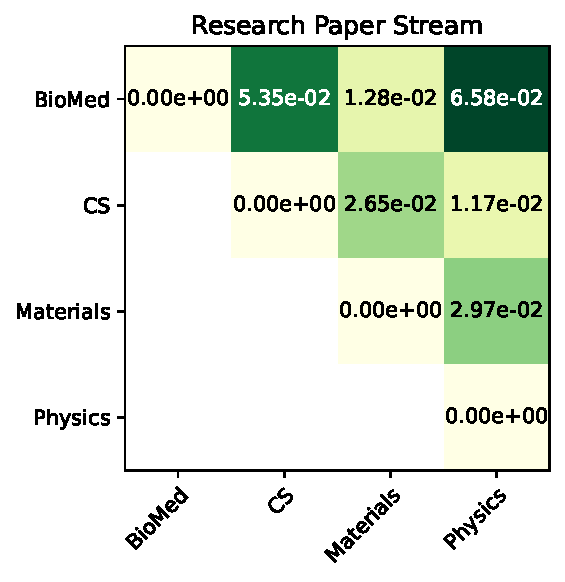
\includegraphics[width=0.80\linewidth]{acl2022/figs/dataset_analysis/sim_paper.pdf}}
    
    \subfloat[\scriptsize{Tweet Stream}]{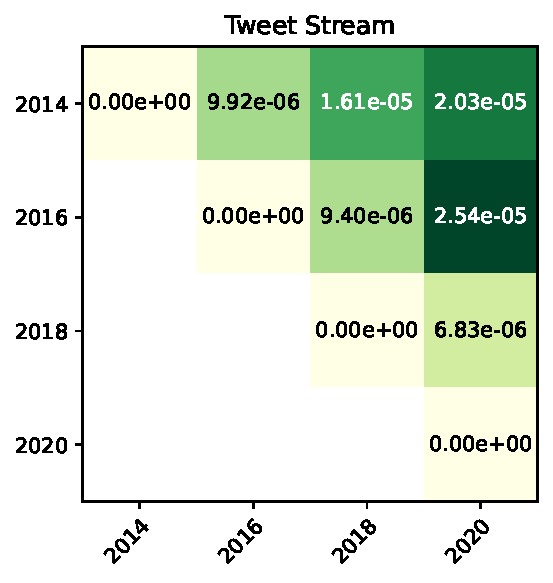
\includegraphics[width=0.80\linewidth]{acl2022/figs/dataset_analysis/sim_tweet.pdf}}

    % }
    \caption{Cosine distance of vocabulary distributions between each pair of datasets in two data streams.}
    \label{fig:vocab_sim_analysis}
\end{figure}

\section{Ethic Risks}
We would like to note that, in practice, continually pretrained models over real-world data streams would require identification and removal of biased contents from pretraining corpora, which may affect the prediction of downstream models. As PTLMs are continuously updated, the bias in earlier pretraining may have a profound negative impact. In future works, it is preferable to develop algorithms to ``forget'' certain biased knowledge from language models. We further note that any data released in this paper, especially the tweet stream, should only be used for research purposes.
% \section{License of RealNews Dataset}

% \begin{table}[]
%     \centering
%     \begin{tabular}{p{10cm}}
% We, the researchers at the University of Washington, provide access to the RealNews dataset as well as the Grover-Mega checkpoints (the resources) under the following conditions. By selecting "I agree" the researcher agrees to the following:

% 1. RealNews and the Grover-Mega checkpoints must only be used for research or education purposes. Use of the resources for malicious purposes, including but not limited to spreading disinformation, explicitly violates this agreement. The resources should not be used for financial gain or profit.
% 2. There is no warranty regarding RealNews or the Grover-Mega checkpoints. We cannot be held liable for providing access to the resources.
% 3. The resources should not be provided to any third party.
% 4. The researcher takes full responsibility for consequences resulting from usage of the provided resources.
% 5. If any part of this agreement is found to be invalid, this should not affect the other parts of the remaining agreement. \\
% \end{tabular}
% \caption{License of the Realnews dataset}

% \label{tab:license_realnews}
% \end{table}



\end{document}
